\documentclass{llncs}
\usepackage{amssymb}
\usepackage{graphicx}
\usepackage[ruled,linesnumbered,boxed]{algorithm2e}
\usepackage{graphicx}
\usepackage{amsmath}
%\usepackage{mathtools}
%\usepackage{color}
\usepackage{tabularx}
\usepackage[colorlinks, linkcolor=blue, anchorcolor=blue, citecolor=green]{hyperref}
%\usepackage{booktabs}
\usepackage[table]{xcolor}
%\uespackage{colortbl}
\usepackage{fancyhdr}
\usepackage{lastpage}
\usepackage{layout}
\usepackage{diagbox}
\usepackage{textcomp}
\usepackage{subcaption}
\usepackage{threeparttable}
\usepackage{booktabs}
\usepackage{multirow}
%\usepackage{ctex}

%\footskip = 10pt
\pagestyle{fancy}
\chead{Group Project}
\lhead{CS214-Algorithm@SJTU}
\rhead{Instructor: Xiaofeng Gao}
\rfoot{}
\cfoot{Page \thepage \ of \pageref{LastPage}}
\addtolength{\headheight}{0.5\baselineskip}
\addtolength{\headwidth}{0\marginparsep}
\addtolength{\headwidth}{0\marginparwidth}



\title{A Design of a Customized Bus-Booking Platform}


\author{Junxiang Cao (518021910574, cjxqaq@sjtu.edu.cn), Sen Li (518021910608, 874049001@qq.com), Shiqu Wu (518021910665, 15759684259@163.com)}
\institute{Department of Computer Science, \\ Shanghai Jiao Tong University, Shanghai, China}

\begin{document}
\bibliographystyle{splncs}

%\linespread{0.85}

%==============================================================================
\maketitle
\begin{abstract}\vspace{-5mm}
The airport traffic problems caused by night flights reflect the need for a bus platform that can respond to orders. The new platform needs to be improved due to the problem of the carrying capacity and cost of taxi.

Our report is to design a static bus order planning scheme. Initially, we set up the virtual airport separately as the starting point of the order, and screen the orders to be calculated within the radius. And we use the $K-means$ clustering algorithm to get the corresponding destinations, and then use genetic algorithm to plan the bus route for the corresponding situation. After consulting the relevant data to determine all the unknown parameters, the profit is counted and compared with taxi.


\textbf{Keywords:} virtual airport, bus, orders, static route planning.
\end{abstract}

\section{Introduction}
\subsection{Problem Background}
With the rapid development of cities and the rapid expansion of population in recent years, the improvement and renewal of urban transportation systems have become a major problem. More and more cities are beginning to popularize the medium and long-distance transportation tools in cities such as subway and light rail. Bicycle sharing also solves many "last mile problems" during commuting, but some groups still have unmet transportation needs.

According to statistics from relevant departments, many passengers arrive at their destinations on late night flights, but due to the suspension of mainstream public transportation such as subway buses, they can only be forced to choose taxis, airport shuttle buses, or the emerging online car rental. However, the carrying capacity of this part of the transportation mode is not ideal enough to satisfy all passengers who arrive at their destination late at night. Therefore, there are areas for improvement in the transportation system.

\subsection{Our Work}
At first, we focus on how to reduce the amount of data used. Thus we want to consider setting up a virtual airport first, and then we use different numbers of destinations, and visualize them.

Then we consider how to design algorithm and dispatch buses to maximum the profit. Of course we do consider the passenger satisfaction factor. After numerical experiments, we have feasible solutions which can be compared with optimal solutions. Finally, we compare it with taxi.


\section{Assumption}
In order to simplify our design work, we make the following assumptions:

\begin{itemize}
	\item Only those data included in virtual airport which we use a circle to build. And all the orders in the circle are considered to start in the at the center of the circle.
	
	\item For each passenger $i$, the bus fare is decided by the linear distance from departure to destination.
	
\end{itemize}

\section{Nomenclature}
In this project we use the nomenclature in Table \ref{tab:Nomen} to descibe our design. 
\begin{table}[h]
	\centering
	\caption{Nomenclature}
	\label{tab:Nomen}
	\fontsize{12}{20}\selectfont
	\begin{tabular}{c c c}
		\hline
		Symbol & Definition & Unit\\
		\hline
		
		$d_i$ & Destination of passenger i & --- \\
		$L$ & Capacity limitation of each bus & --- \\
		$c_b$ & Bus fuel cost per kilometer & $yuan$\\
		$c_r$ & Cost per route of a bus &  $yuan$ \\
		$p_i$ & Bus fare price to station $d_i$  &  $yuan$ \\	
		$r_i$ & Route length of bus $i$  &  $kilometer$ \\	
		$P$ & Profit  &  $yuan$ \\
		
		\hline
	\end{tabular}
\end{table}

\section{Design Task with Numerical Experiments}
\subsection{Virtual Airport Selection}
First we need to set virtual airport based on the departure location of orders.

\begin{enumerate}
	\item \textbf{Chengdu}. In Chengdu, it is easy to determine where the virtual airport should be. Chengdu is a city centered on Tianfu Square. Therefore it is very suitable to set up a virtual airport with Tianfu Square as the center. Fig.\ref{fig-chengdu-start} shows the obvious center of Chengdu both in geography and in our orders. We set virtual airport with a radius of $3.4$ kilometers.
	
		\begin{figure}[h]
		\centering
		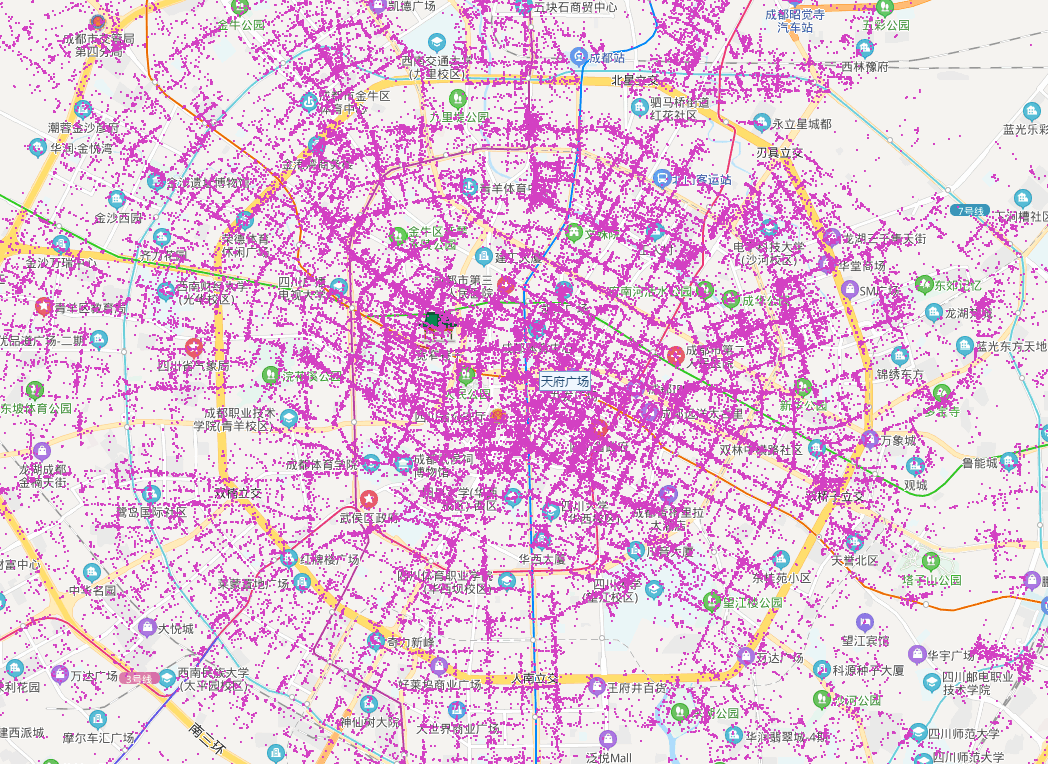
\includegraphics[width=1\textwidth]{figures/chengdu_start.png}
		\caption{Departure nodes map of Chengdu}
		\label{fig-chengdu-start}
	    \end{figure}
 
 	\item \textbf{Haikou}. In Haikou, it is not obvious to determine the virtual airport as shown in Fig.\ref{fig-haikou-start}. 
 	
 		\begin{figure}[h]
 		\centering
 		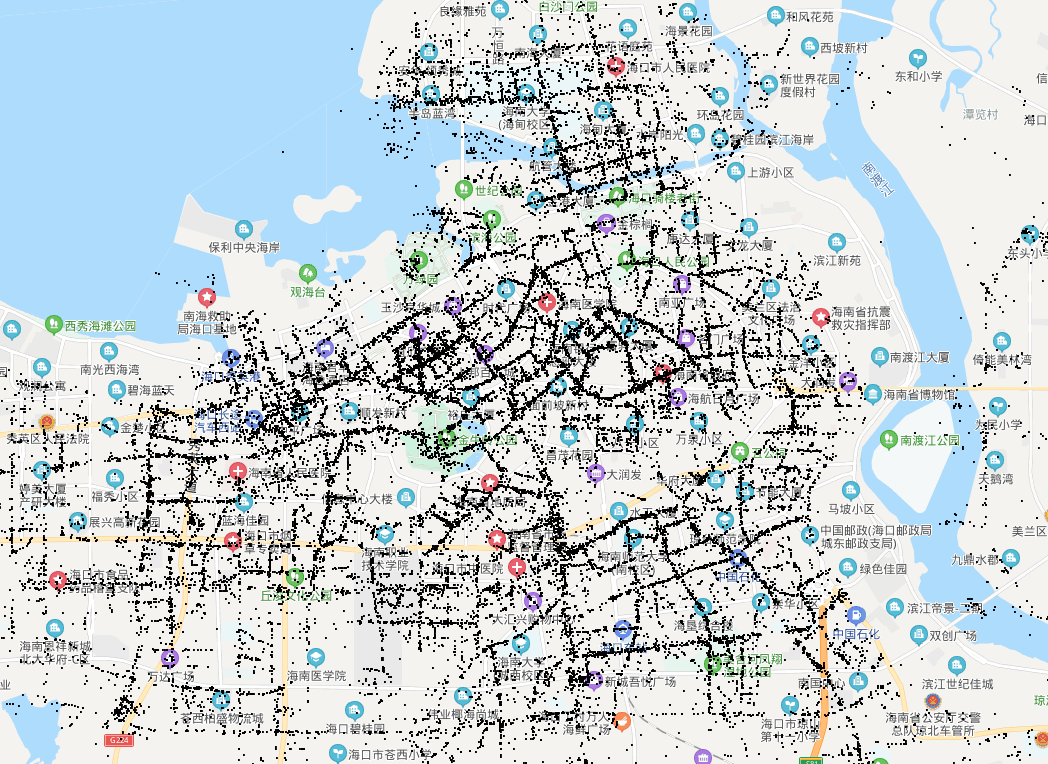
\includegraphics[width=1\textwidth]{figures/haikou_start.png}
 		\caption{Departure nodes map of Haikou}
 		\label{fig-haikou-start}
 		\end{figure}

 	
 	So we first pick $5$ high order density landmark, which is shown in Table.\ref{tab-hainan}.
 	
 	\begin{table}[htbp]
 			\caption{$5$ Landmarks With High Oeder Density}
 		\begin{center}
 			\begin{tabular}{|c|c|c|}
 				\hline
 				\diagbox[width=30em,trim=l]{Landmark}{Value}{Column} & Longitude(°E) & Latitude(°N)  \\
 				\hline
 				Hainan Provincial Government							 & $110.3543$ & $20.0241$\\
 				\hline
 				Hainan Medical College      							 & $110.3366$ & $20.0345$\\
 				\hline
 				Haikou Intermediate People's Court    				     & $110.3348$ & $20.0237$\\
 				\hline
 				Haikou Hospital of traditional Chinese Medicine          & $110.3336$ & $19.9941$\\
 				\hline
 				Haikou Coach West Station          					     & $110.2976$ & $20.0175$\\
 				\hline
 			\end{tabular}
 		\end{center}
 		\label{tab-hainan}
 	\end{table}
Then we calculate the average longitude and latitude of these $5$ landmarks and get the location of the virtual airport which is ($110.3314$°E,$20.0188$°N). And then we screen out the orders in the virtual airport with a radius of $4$ kilometers.
 	
\end{enumerate}
\subsection{Destination Selection}
To select some hot node as our bus destinations, we need to consider the destination denisty among all the orders we consider. In order to get a more representative destination, we decide to adopt $k-means$ clustering algorithm. To better explain it, we use pseudocode in Alg.\ref{alg-1}.

\begin{minipage}[t]{0.8\textwidth}
	\begin{algorithm}[H]
		\label{alg-1}
		\KwIn{Number of samples $n$, cluster number $k$ and initial cluster center $\mu_1,\mu_2,\cdots,\mu_n$}
		\KwOut{Final clustering center (destinations) $\mu_1,\mu_2,\cdots,\mu_n$}
		\BlankLine
		\caption{$k-means$ clustering algorithm}
		
		\Repeat{$\mu_1,\mu_2,\cdots,\mu_n$ do not change}{
		assign the $n$ samples according to the nearest $\mu_i$\;
		recalculate cluster center $\mu_1,\mu_2,\cdots,\mu_k$\;
		}
		\textbf{output} final $\mu_1,\mu_2,\cdots,\mu_k$\;
	\end{algorithm}
\end{minipage}

After $k-means$ cluster algorithm, we can get $k$ hot destinations. There are two versions of $k=30$ and $k=50$. And for both Chengdu and Haikou, we both get the final destinations in Fig.\ref{fig-k}.

\begin{figure}[htbp]
	\centering
	\begin{subfigure}[t]{0.45\textwidth}
		\begin{minipage}{6cm}
			\centering
			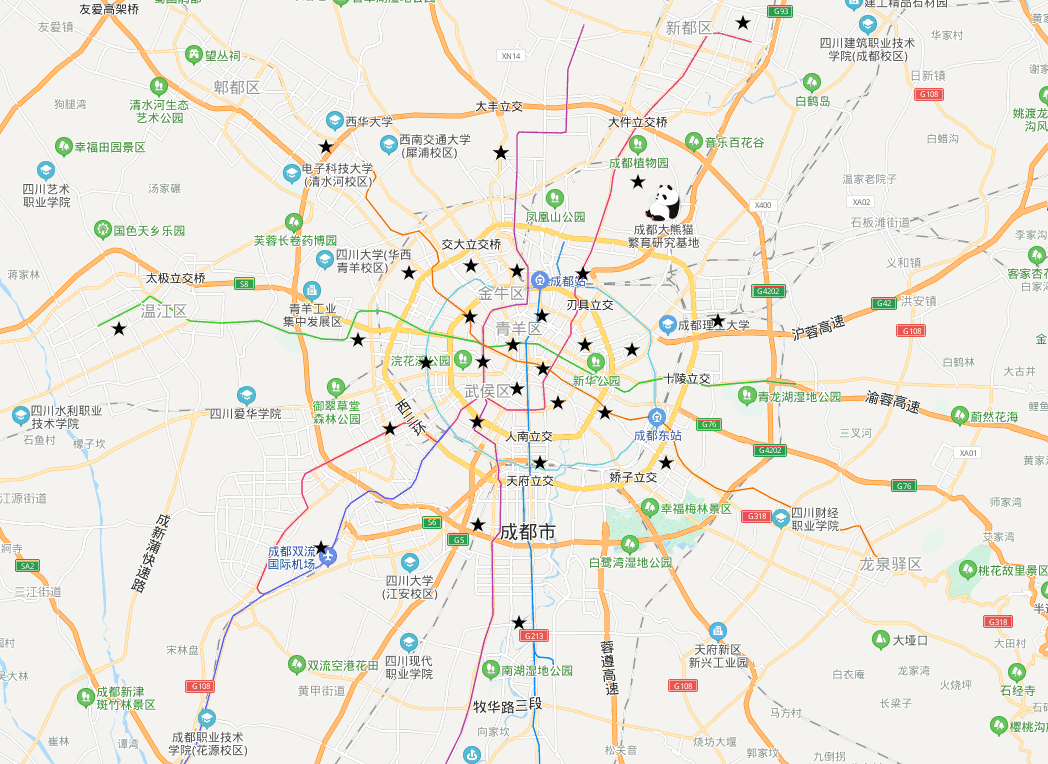
\includegraphics[width=6cm]{figures/chengdu_30.png}
			\caption{30 Clusting Destinations of Chengdu}
		\end{minipage}%
	\end{subfigure}
	\begin{subfigure}[t]{0.45\textwidth}
		\begin{minipage}{6cm}
			\centering
			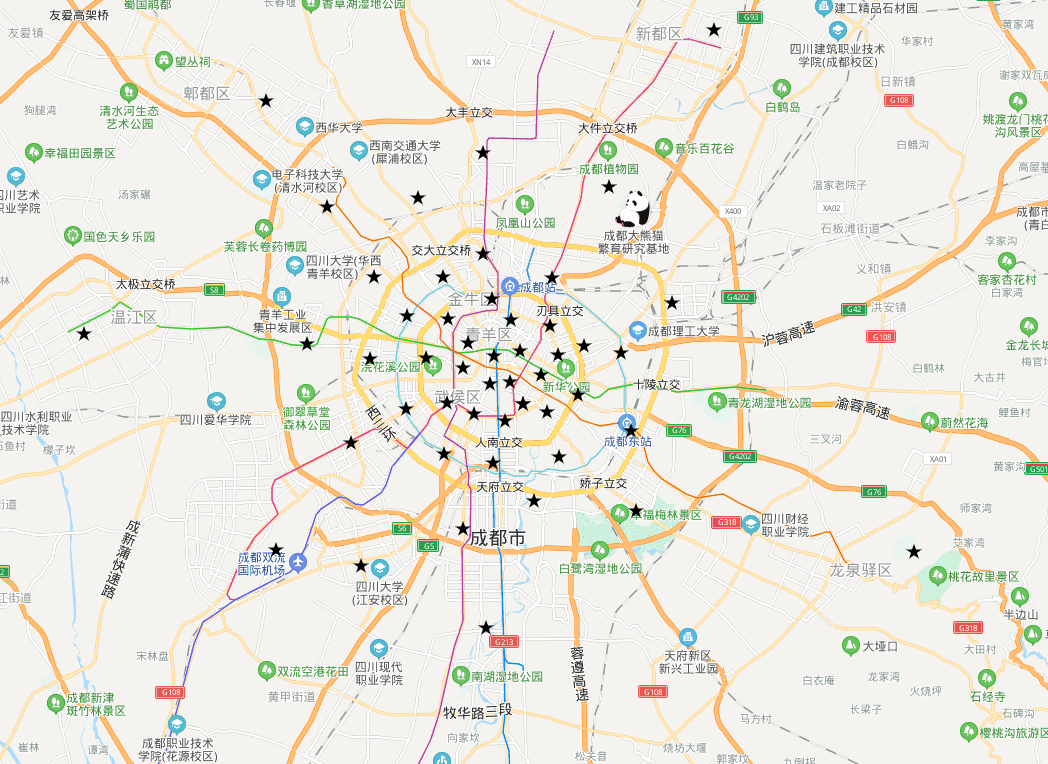
\includegraphics[width=6cm]{figures/chengdu_50.png}
			\caption{50 Clusting Destinations of Chengdu}
		\end{minipage}
	\end{subfigure}
	\begin{subfigure}[t]{0.45\textwidth}
		\begin{minipage}{6cm}
			\centering
			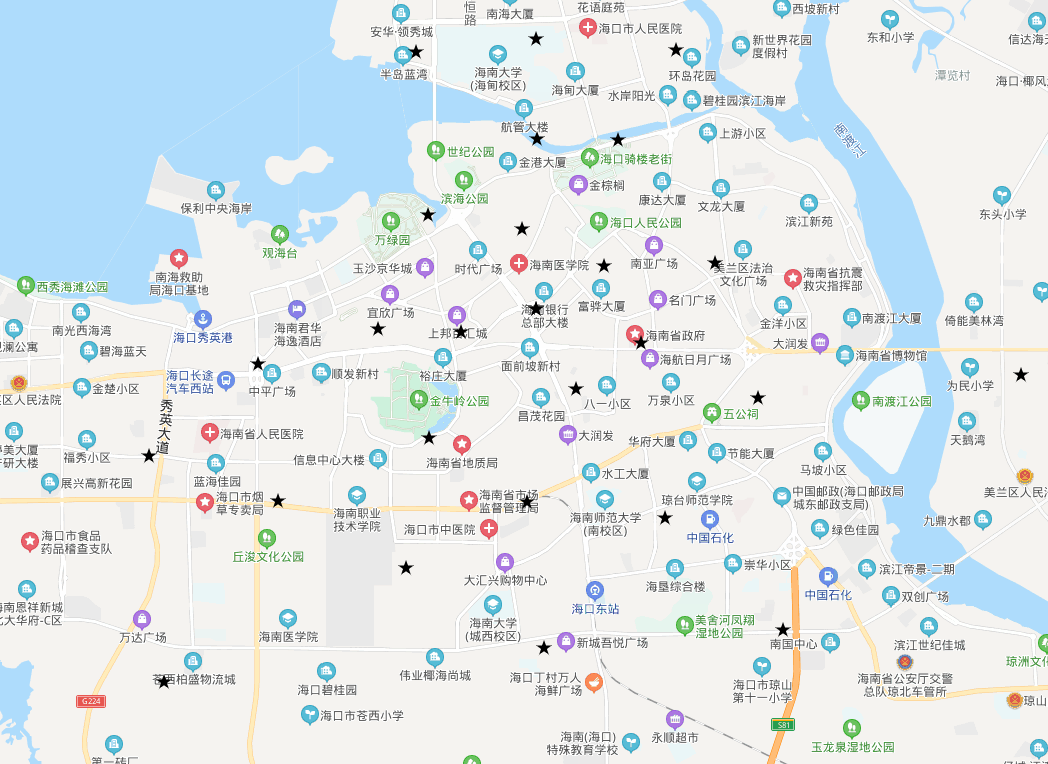
\includegraphics[width=6cm]{figures/haikou_30.png}
			\caption{30 Clusting Destinations of Haikou}
		\end{minipage}%
	\end{subfigure}
	\begin{subfigure}[t]{0.45\textwidth}
		\begin{minipage}{6cm}
			\centering
			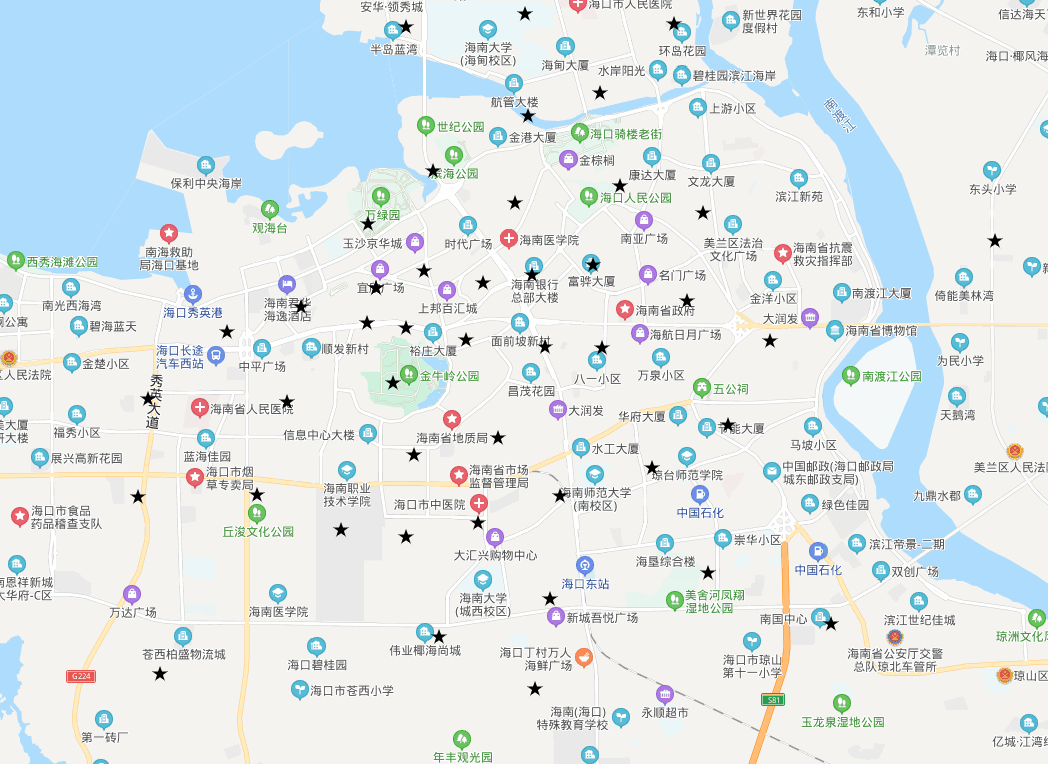
\includegraphics[width=6cm]{figures/haikou_50.png}
			\caption{50 Clusting Destinations of Haikou}
		\end{minipage}
	\end{subfigure}
	\caption{$k-means$ Clusting Destinations Map}
	\label{fig-k}
\end{figure}

\subsection{Problem Formulation}
Here we give the formal defnitions of three ODRP problems.
\begin{enumerate}
	\item Suppose that there are $n$ passengers and $m$ buses at the departure station, while the destination station of passenger $i$ is $d_i\in D$ and the capacity limitation of each bus is $L$. The bus fuel cost per kilometer is $c_b$. The cost per route of a bus is $c_r$. The bus fare price for one passenger from the departure station to station $d_j$ is $p_j$. Please dispatch each bus $i$ with a route whose length is $r_i$ kilometers to satisfy all passengers ($n < mL$) and maximum the profit $P = \sum_{i=1}^{n}p_i -\sum_{i=1}^{m}c_r - \sum_{i=1}^{m}(c_b\times r_i)$.
	
	\item Suppose that there are $n$ passengers and $m$ buses at the departure station, while the destination station of passenger $i$ is $d_i\in D$ and the capacity limitation of each bus is $L$. The bus fuel cost per kilometer is $c_b$. The cost per route of a bus is $c_r$. The bus fare price for one passenger from the departure station to station $d_j$ is $p_j$. Please dispatch each bus $i$ with a route whose length is $r_i$ kilometers to but do not need to satisfy all passengers (suppose satisfying $x$ passengers) and only in order to maximum the profit $P = \sum_{i=1}^{x}p_i -\sum_{i=1}^{m}c_r - \sum_{i=1}^{m}(c_b\times r_i)$.
	
	\item Suppose that there are $n$ passengers and $m$ buses at the departure station, while the destination station of passenger $i$ is $d_i\in D$ and the capacity limitation of each bus is $L$. The bus fuel cost per kilometer is $c_b$. The cost per route of a bus is $c_r$. The bus fare price for one passenger from the departure station to station $d_j$ is $p_j$. Please dispatch each bus $i$ with a route whose length is $r_i$ kilometers to but do not need to satisfy all passengers (suppose drop off $y$ passengers and it will lead to losing $\alpha y$ more potential passengers) and  in order to maximum the profit $P = \sum_{i=1}^{n-y-\alpha y}p_i -\sum_{i=1}^{m}c_r - \sum_{i=1}^{m}(c_b\times r_i)$.
	
\end{enumerate}
\subsection{Algorithm Design}
\textbf{Brief Explanation of Genetic Algorithm in Path Planning:} For ODRP-V2 problem, since in section 2.1 we've select the $k$ hot destinations, we view them as points (dusbins) here. Our goal is to maximize the total profit of STMB, which is to say: minimize the total distance of routes (since the car maintanence fee per route is a constant $c_r$ , the fule cost per car per kilometer is also a constant $c_b$ and we don't need to concern about the customer's dissatisfaction factor here) while meet the restriction ($m$ bus and each bus's limitation is $L$, so we can take at most $m*L$ customer). In order to meet the goal, we need to let each bus takes as many customers as possible and try to dispatch routes for all the buses (since $n>mL$). It's obvious that each bus's route will not contaion the same vertex twice, after it has reached its last destination station or all the customers in the bus have been delivered properly, the shortest path is to directly go back to the departure station. These features are the same as Multiple Traverling Salesman's Problem (we use MTSP to represent it in the following part). Therefore, we consider to use Genetic Algorithm to solve route planning problem because it's a typical, widely used method to solve MTSP. There are five main metrics of GA: gene, chromosome, individual,population and fitness. Each of these five metrics is corresponding to separated stations, route, one bus dispatching, all $m$ buses route dispatching, total geometry distance for each route. Since it's very convenient to use a sequence of numbers to represent a route, where each number represents a separated station, it's easy to construct chromosome, which is convenient for our later operation. And there are three main steps of GA:
\begin{itemize}
\item Step one: Calculate the fitness of each individual of current population and do the selection according to the selection rules (we use tournament selection here) to form a new generation .

\item Step two: Perform crossover in some rate on each indivisuals. When two individuals are selected in crossover steps, exchange their chromosomes(exchange some stations in the route) using the cross strategy.

\item Step three: Do the mutation in some rate on each indivisuals. When the individual is selected to do the mutation, remove some stations from the route and add new stations.
\end{itemize}

\subsection{Pricing Strategy}
We tend to charge by mileage, that is, the distance from the Department to the passenger's destination is directly proportional to the custom fare. At the same time, we introduce the fare gap parameter, that is, the difference $p$ between our pricing and taxi price, as the fare gap parameter. The smaller the fare gap, the lower the parameter, which means that the higher the fare, the smaller the probability of passengers willing to choose our bus system. Our goal is to find the extreme point in the middle.

At first, we need to show the data of simple bus and taxi price strategy in both Chengdu and Haikou to better determine our special bus price. Here is shown in Tab.\ref{tab-tb}.

	\begin{table}[htbp]
	
	\centering
	\fontsize{13}{19}\selectfont 
	\begin{threeparttable}
		\caption{Price strategy of taxi and simple bus system}
		\label{tab-tb}
		\begin{tabular}{ccccccc}
			\toprule
			\multirow{2}{*}{Category}&
			\multicolumn{3}{c}{Chengdu}&\multicolumn{3}{c}{Haikou}\cr
			\cmidrule(lr){2-4} \cmidrule(lr){5-7}
			&Taxi(starting)&Taxi(extra $/km$)&Bus&Taxi(starting)&Taxi(extra $/km$)&Bus\cr
			\midrule
			{\bf Day(taxi)}   &$8$&$1.9$(2-10km) $2.9$(10-60km)&-----&$8$&$2$(2-10km)&-----\cr
			{\bf Night(taxi)} &$9$&$2.2$(2-10km) $3.3$(10-60km)&-----&-----&-----&-----\cr
			{\bf Day(bus)}    &-----&-----&$2$&-----&-----&$2$\cr
			{\bf Night(bus)}  &-----&-----&$3$&-----&-----&$2$\cr
			\bottomrule
		\end{tabular}
	\end{threeparttable}
	\end{table}

Our special bus price need to be one value between simple bus and taxi. So here we introduce a $P$ function to express the price strategy.  Fig.\ref{fig-p} shows how the $P$ function determins.

\begin{figure}[h]
	
	\centering
	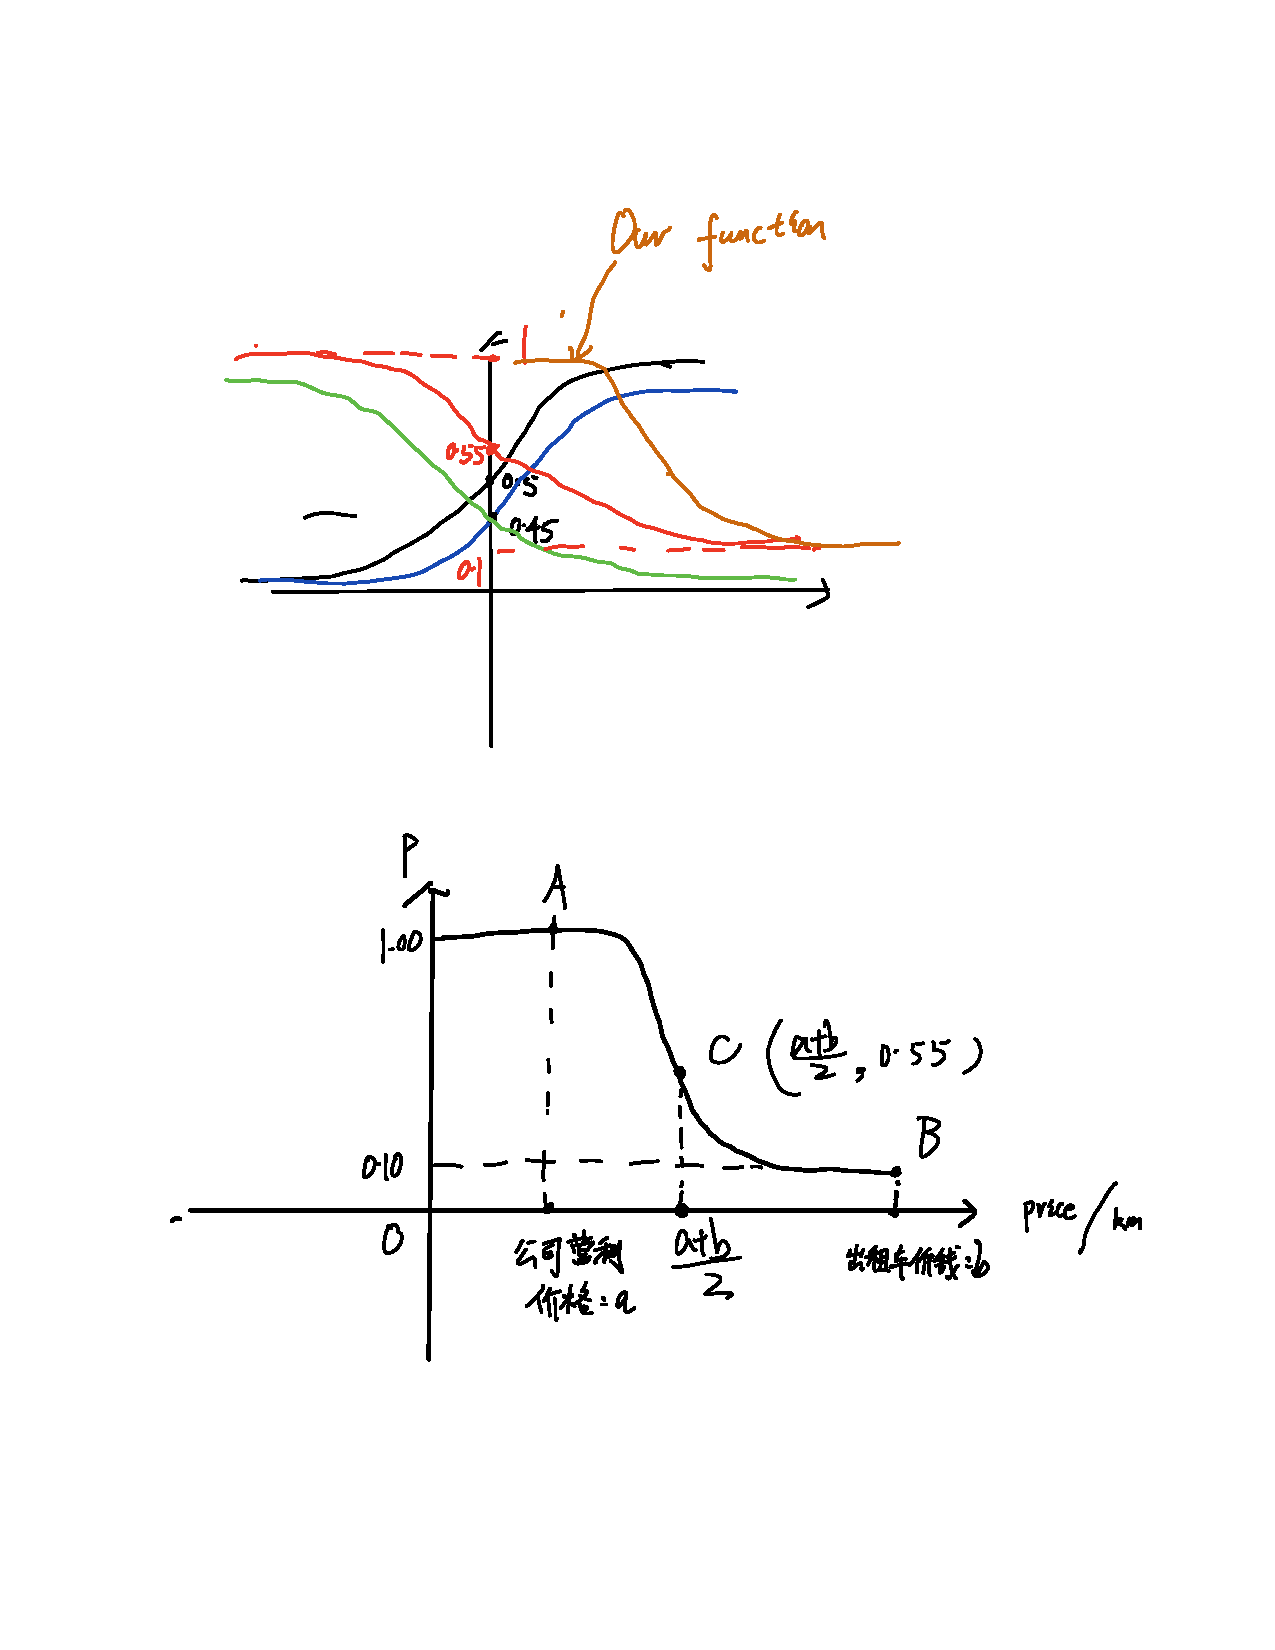
\includegraphics[width=12cm]{figures/Pfunction.pdf}
	\caption{P Function Foramtion}
	\label{fig-p}
	
\end{figure}

The key step is how to we determine $A$ and $B$.
\begin{itemize}
	\item \textbf{Node A}. Assume our bus system price (which will not earn or lose) will not bore customers at all. At this time, $P=1$.
	
	\item \textbf{Node B}. Assume our price goes highest at taxi price, and due to carpooling factors, most passengers are unwilling to choose our bus system. But there is still part of them will choose our bus system (assume the ratio is $10\%$) because of their waiting bus is ready at departure or they are a small group of more than four people (more than taxi load). Due to the S-shaped change of customer purchasing psychology index about commodity price, we set $sigmoid$ function as our $P-price$ function, which is $a-\frac{1}{c(a+e^{-d(x-e)})}$. After solving, we can get $P(x) = 1-\frac{1}{1.12(1+e^{-d(x-\frac{a+b}{2})})}$. After the specific value is brought in, the mathematical expression is as follows:
	
	\begin{equation*}
		P(x) = 1-\frac{1}{1.12(1+e^{-3.53(x-1.38)})} (0.068 < x < 3.3)
	\end{equation*}
	$x$ means our bus fare per kilometer, $0.068$ is the lower limit to earn profit and $3.3$ is the night taxi fare. $P$ function is like the probability function which reflects the willingness of passengers to choose our bus system. We roughly divide several points to test the change of customer satisfaction. Details are shown in Tab.\ref{tab-pfunction}.
	
	 	\begin{table}[htbp]
	 				\caption{Satisfaction $P(x)$ Change Table}
		\begin{center}
			\begin{tabular}{|c|c|c|c|c|c|c|c|}
				\hline
				\diagbox[width=15em,trim=l]{Satisfaction}{fare($x$)} & $0.068$ & $1$ & $1.5$ & $2$ & $2.5$ & $3$ & $3.3$ \\
				\hline
				$P(x)$			& $0.99$ & $0.81$ & $0.46$ & $0.197$ & $0.124$ & $0.11$ & $0.108$\\
				\hline
			\end{tabular}
		\end{center}
		\label{tab-pfunction}
	\end{table}
\end{itemize}

In reality, we can not only consider profits from business, but also customer satisfaction. In fact, when the customer satisfaction is lower than $0.8$, it is very unfriendly to the reputation of our bus system. Therefore, we do not consider the case of less than $0.8$, only looking for a huge profit solution in the satisfaction of more than $0.85$. That is to say, we consider to find solution near $x=1$, we then devide another several points to test  the profit and finally the best price strategy is $0.9yuan/km$. Then $P(x) = 8 + (x-2)\times 0.9 + 1.8$, which $8$ is the flag-down fare of first $2$km.

\subsection{Route Planning and Solution}
\subsubsection{Optimal Solution}
For optimal solution, we use \emph{CPlex} to help solve it. And it is much harder than we think. We change a lot of codes but the computing power is not so ideal that only can calculate up to $30$ orders. Details are as Tab.\ref{tab-optimal}.

	 	\begin{table}[htbp]
			\caption{Optimal Solution of $30$ Orders}
			\begin{center}
			\begin{tabular}{|c|l|}
			\hline
			Category & Value \\
			\hline
			Bus Number	   & $2$ \\
			\hline
			Orders Number	& $30$ \\
			\hline
			$c_b$			& $2$yuan \\
			\hline
			$c_r$			& $5.2$yuan \\
			\hline
			$L$			    & $12$ \\
			\hline
			Total Fuel Fee			& $4$yuan \\
			\hline
			Total Maintenence Cost		& $19.217$yuan \\
			\hline
			Total Income			& $212.48$yuan \\
			\hline
			Profit			& $189.2$yuan \\
			\hline
			\end{tabular}
			\end{center}
	\label{tab-optimal}
		\end{table}

After testing, our optimal solution calculating power's upper limit is $30$ destinations, $25$ carry capacity, $170$ orders, which will cost more than half an hour to get the solution.
\subsubsection{Feasible Solution}
We implement the genetic algorithm designed above and implement it with code, and then substitute it into our order data. The iterative process in the algorithm is as Fig.\ref{fig-it}.

\begin{figure}[htbp]
	\centering
	\begin{subfigure}[t]{0.45\textwidth}
		\begin{minipage}{6cm}
			\centering
			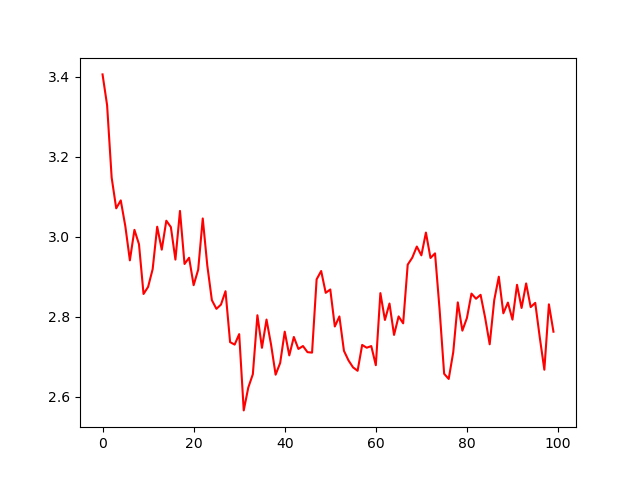
\includegraphics[width=6cm]{figures/cd_30.png}
			\caption{30 Destinations iterating of Chengdu}
		\end{minipage}%
	\end{subfigure}
	\begin{subfigure}[t]{0.45\textwidth}
		\begin{minipage}{6cm}
			\centering
			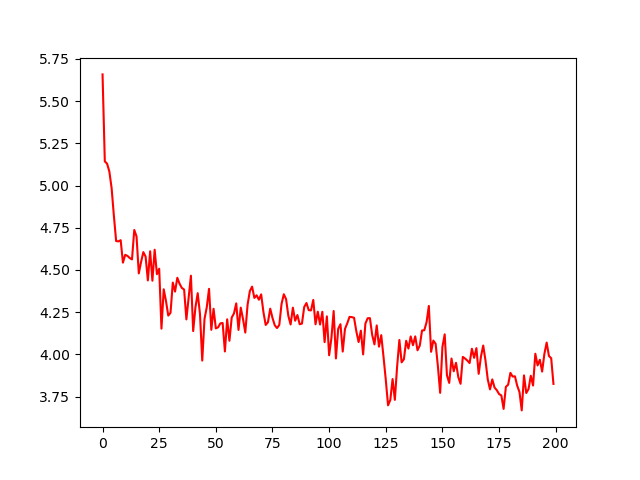
\includegraphics[width=6cm]{figures/cd_50.png}
			\caption{50 Destinations iterating of Chengdu}
		\end{minipage}
	\end{subfigure}
	\begin{subfigure}[t]{0.45\textwidth}
		\begin{minipage}{6cm}
			\centering
			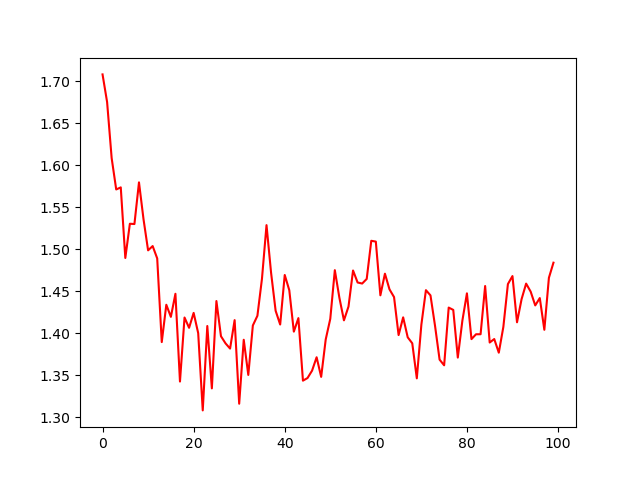
\includegraphics[width=6cm]{figures/hk_30.png}
			\caption{30 Destinations iterating of Haikou}
		\end{minipage}%
	\end{subfigure}
	\begin{subfigure}[t]{0.45\textwidth}
		\begin{minipage}{6cm}
			\centering
			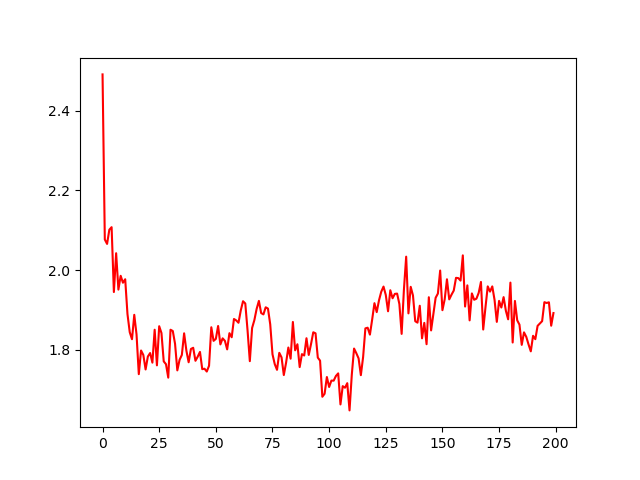
\includegraphics[width=6cm]{figures/hk_50.png}
			\caption{50 Destinations iterating of Haikou}
		\end{minipage}
	\end{subfigure}
	\caption{Genetic Algorithm Iterative Graph}
	\label{fig-it}
\end{figure}

And the final bus route plan is as follows:
\begin{itemize}
	\item \textbf{Chengdu-30}. When $k=30$, there are $5$ bus routes as Fig.\ref{fig-cd-30}.
	
	\begin{figure}[htbp]
		\centering
		\begin{subfigure}[t]{0.45\textwidth}
			\begin{minipage}{6cm}
				\centering
				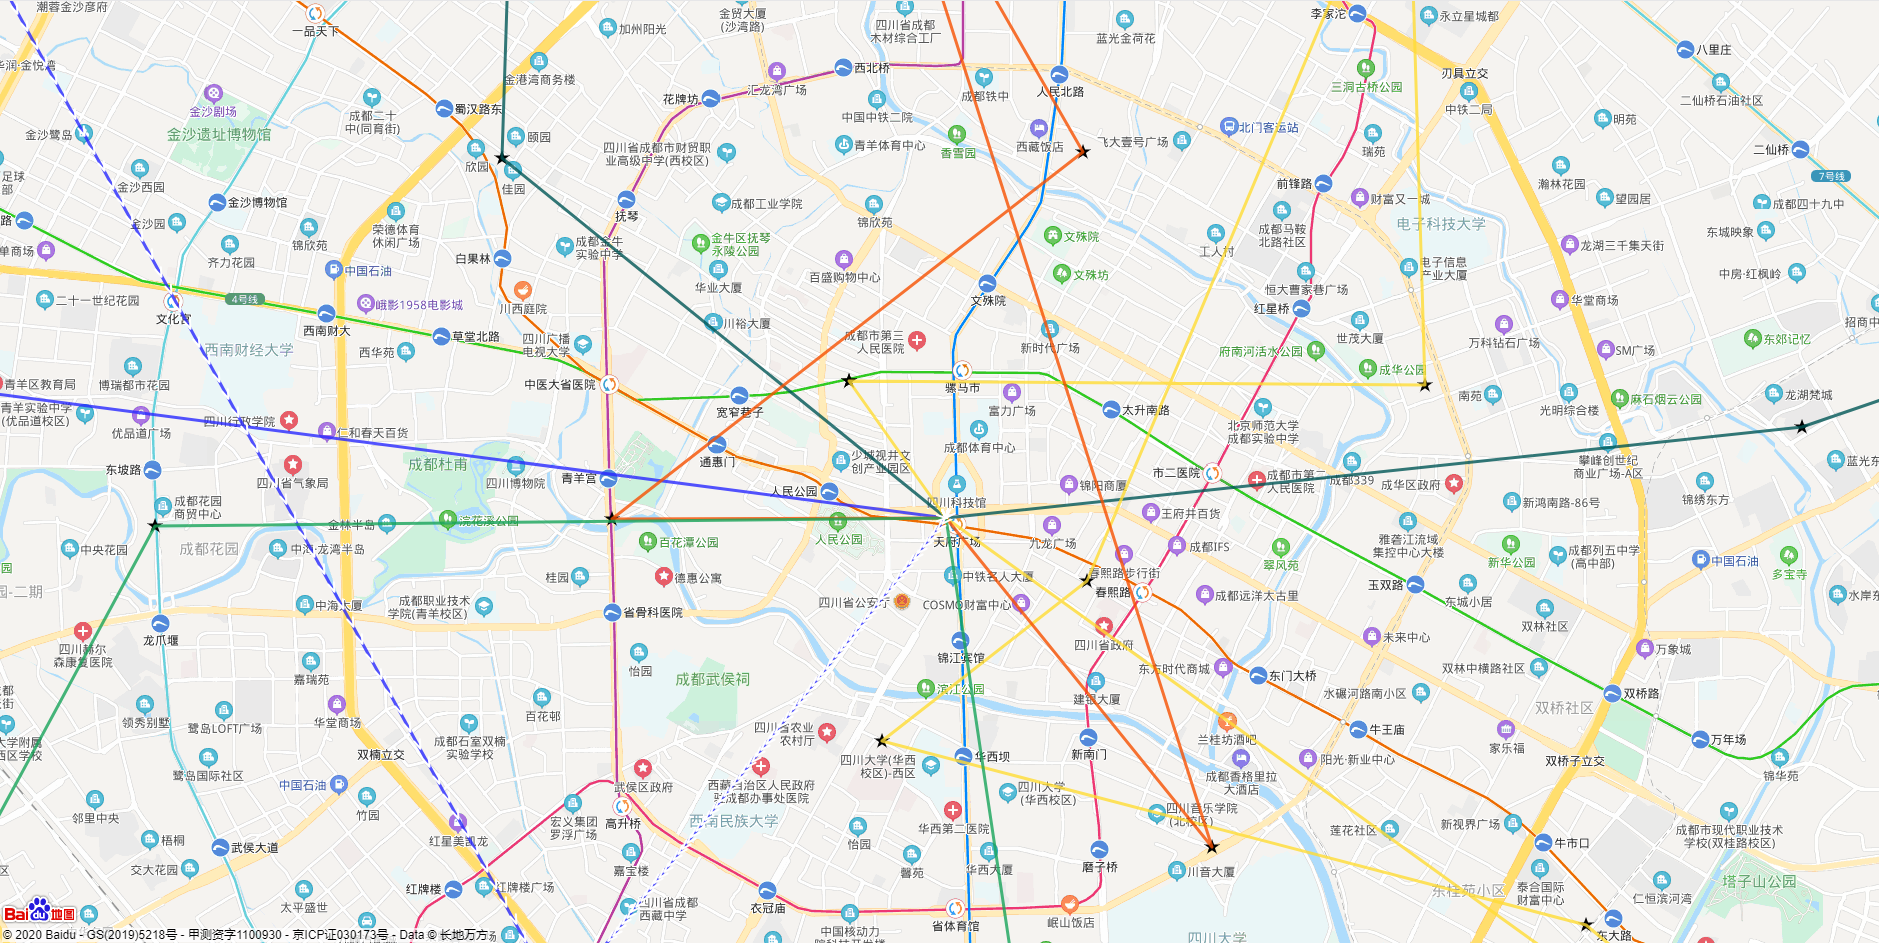
\includegraphics[width=6cm]{figures/cd_30_1.png}
				\caption{Routes Map 1}
			\end{minipage}%
		\end{subfigure}
		\begin{subfigure}[t]{0.45\textwidth}
			\begin{minipage}{6cm}
				\centering
				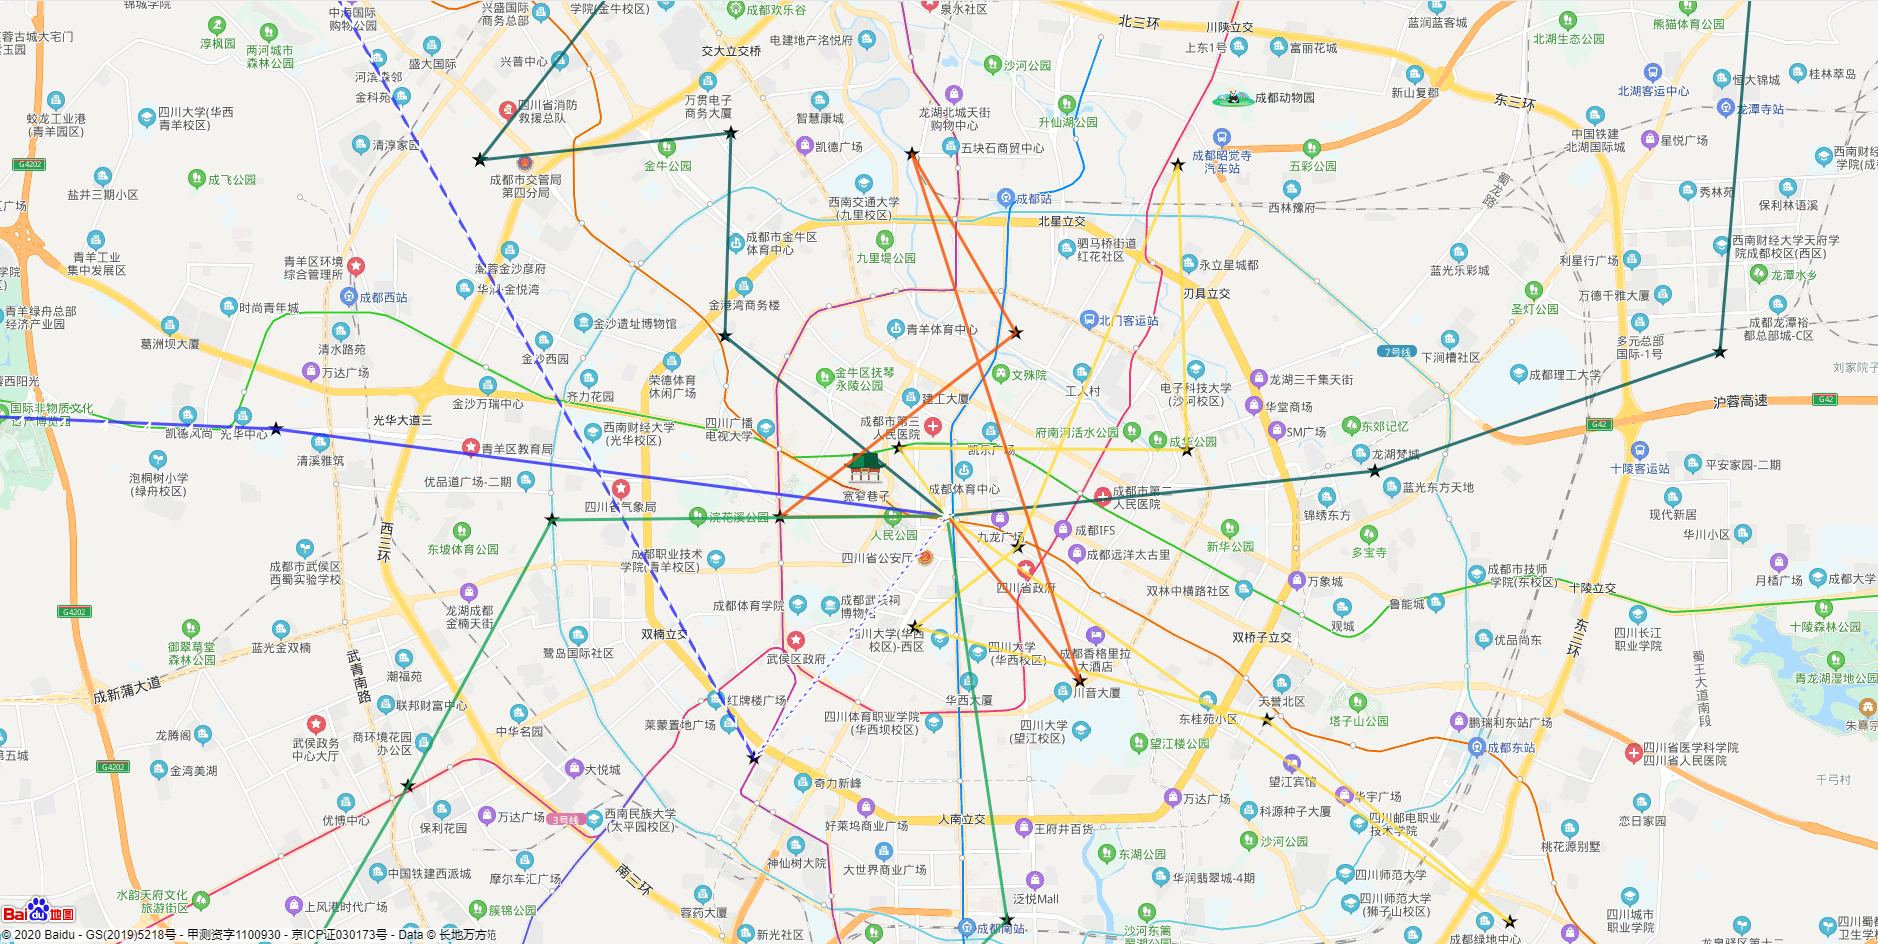
\includegraphics[width=6cm]{figures/cd_30_2.png}
				\caption{Routes Map 2}
			\end{minipage}
		\end{subfigure}
		\begin{subfigure}[t]{0.45\textwidth}
			\begin{minipage}{6cm}
				\centering
				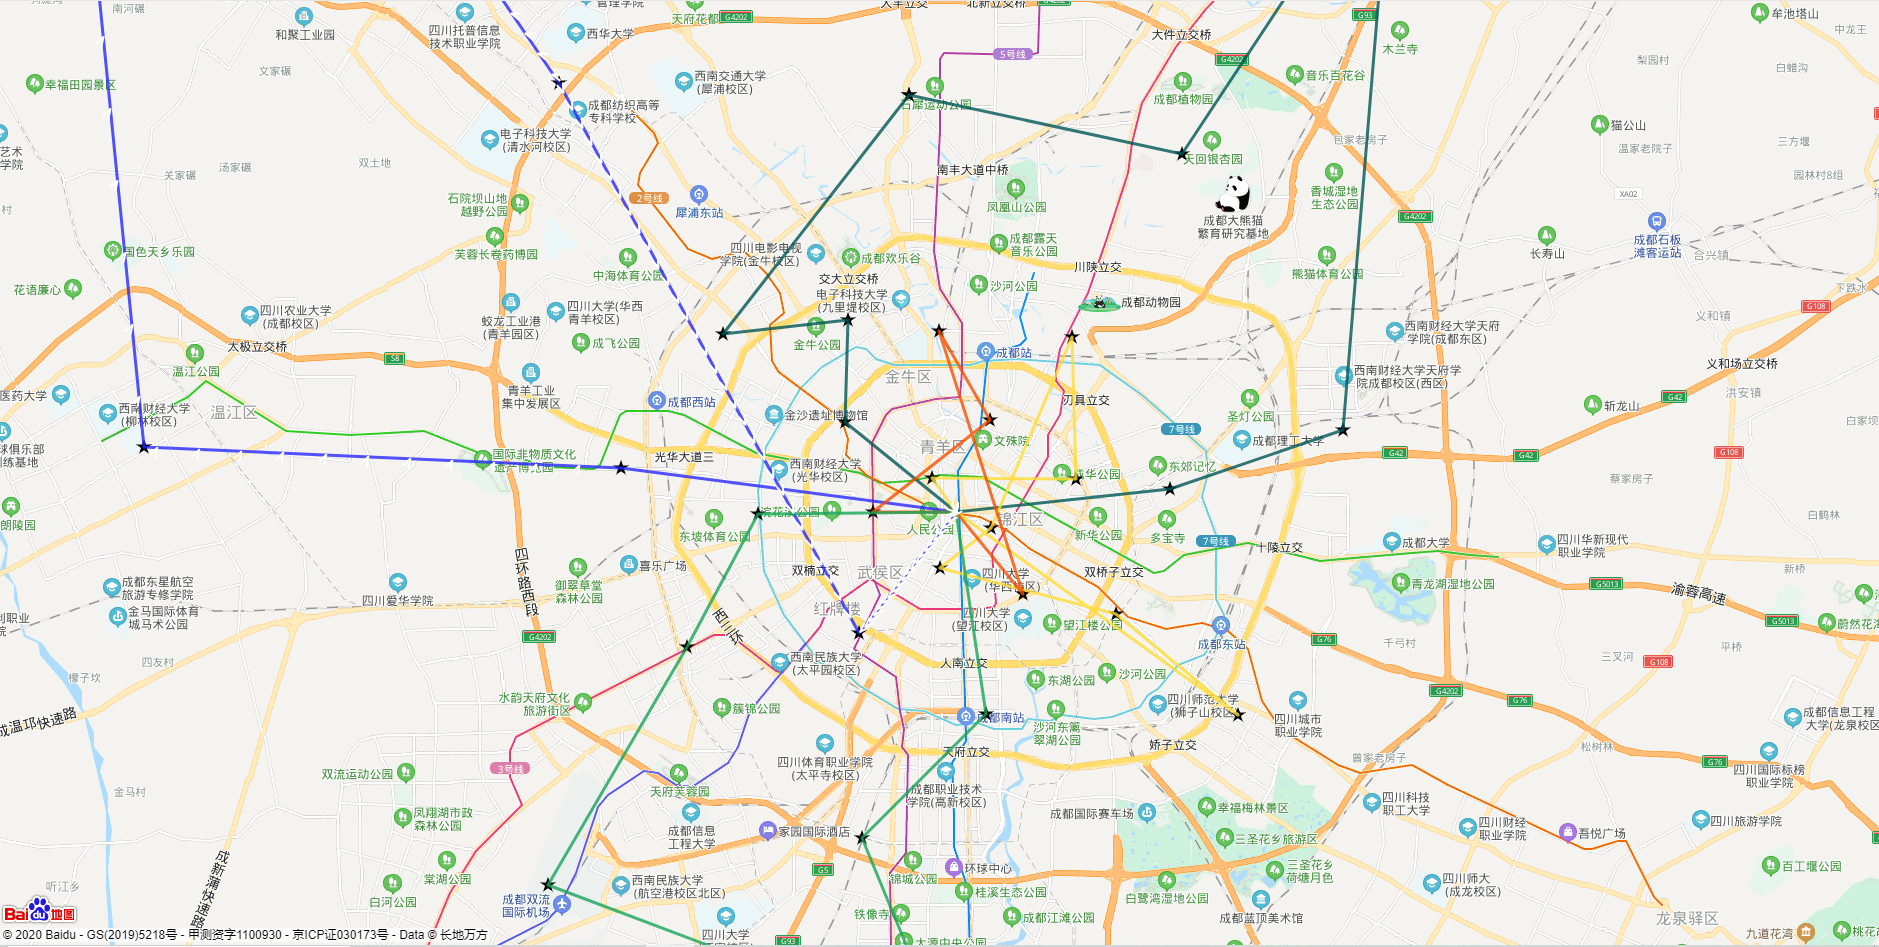
\includegraphics[width=6cm]{figures/cd_30_3.png}
				\caption{Routes Map 3}
			\end{minipage}%
		\end{subfigure}
		\begin{subfigure}[t]{0.45\textwidth}
			\begin{minipage}{6cm}
				\centering
				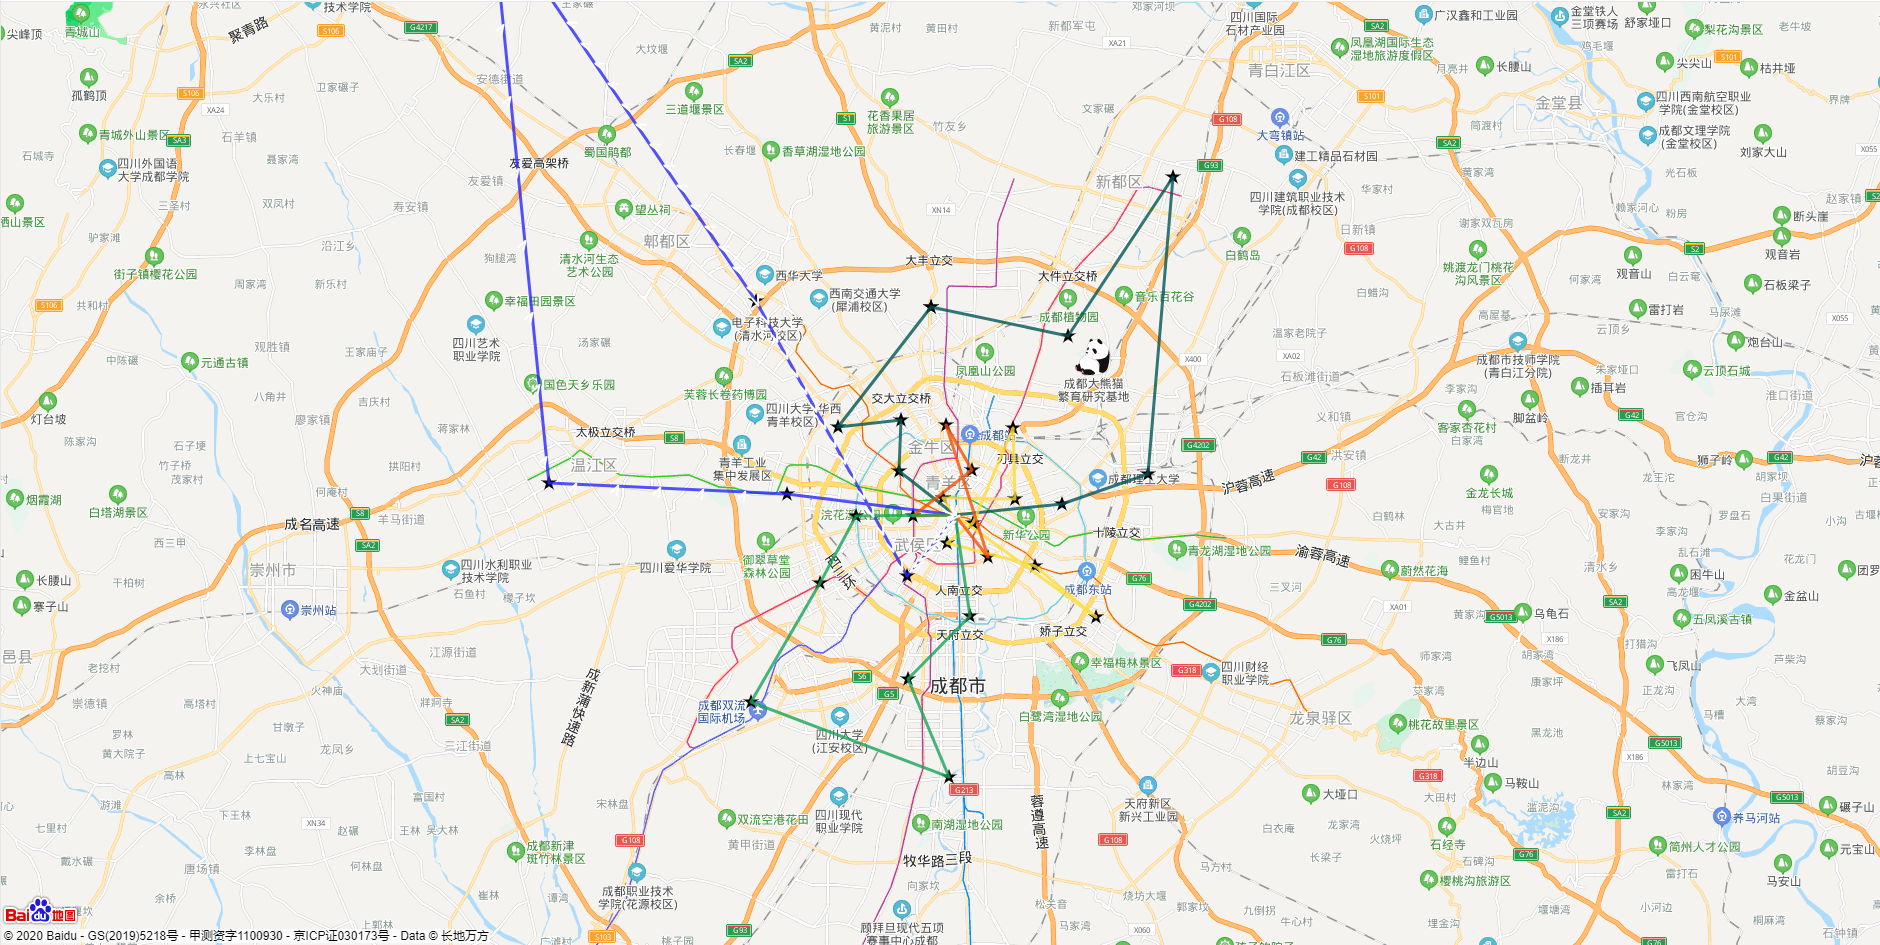
\includegraphics[width=6cm]{figures/cd_30_4.png}
				\caption{Routes Map 4}
			\end{minipage}
		\end{subfigure}
		\caption{$30$ Destinations Routes Maps with Different Scaling of Chengdu}
		\label{fig-cd-30}
	\end{figure}

	\item \textbf{Chengdu-50}. When $k=50$, there are $7$ bus routes as Fig.\ref{fig-cd-50}.

		\begin{figure}[htbp]
		\centering
		\begin{subfigure}[t]{0.45\textwidth}
			\begin{minipage}{6cm}
				\centering
				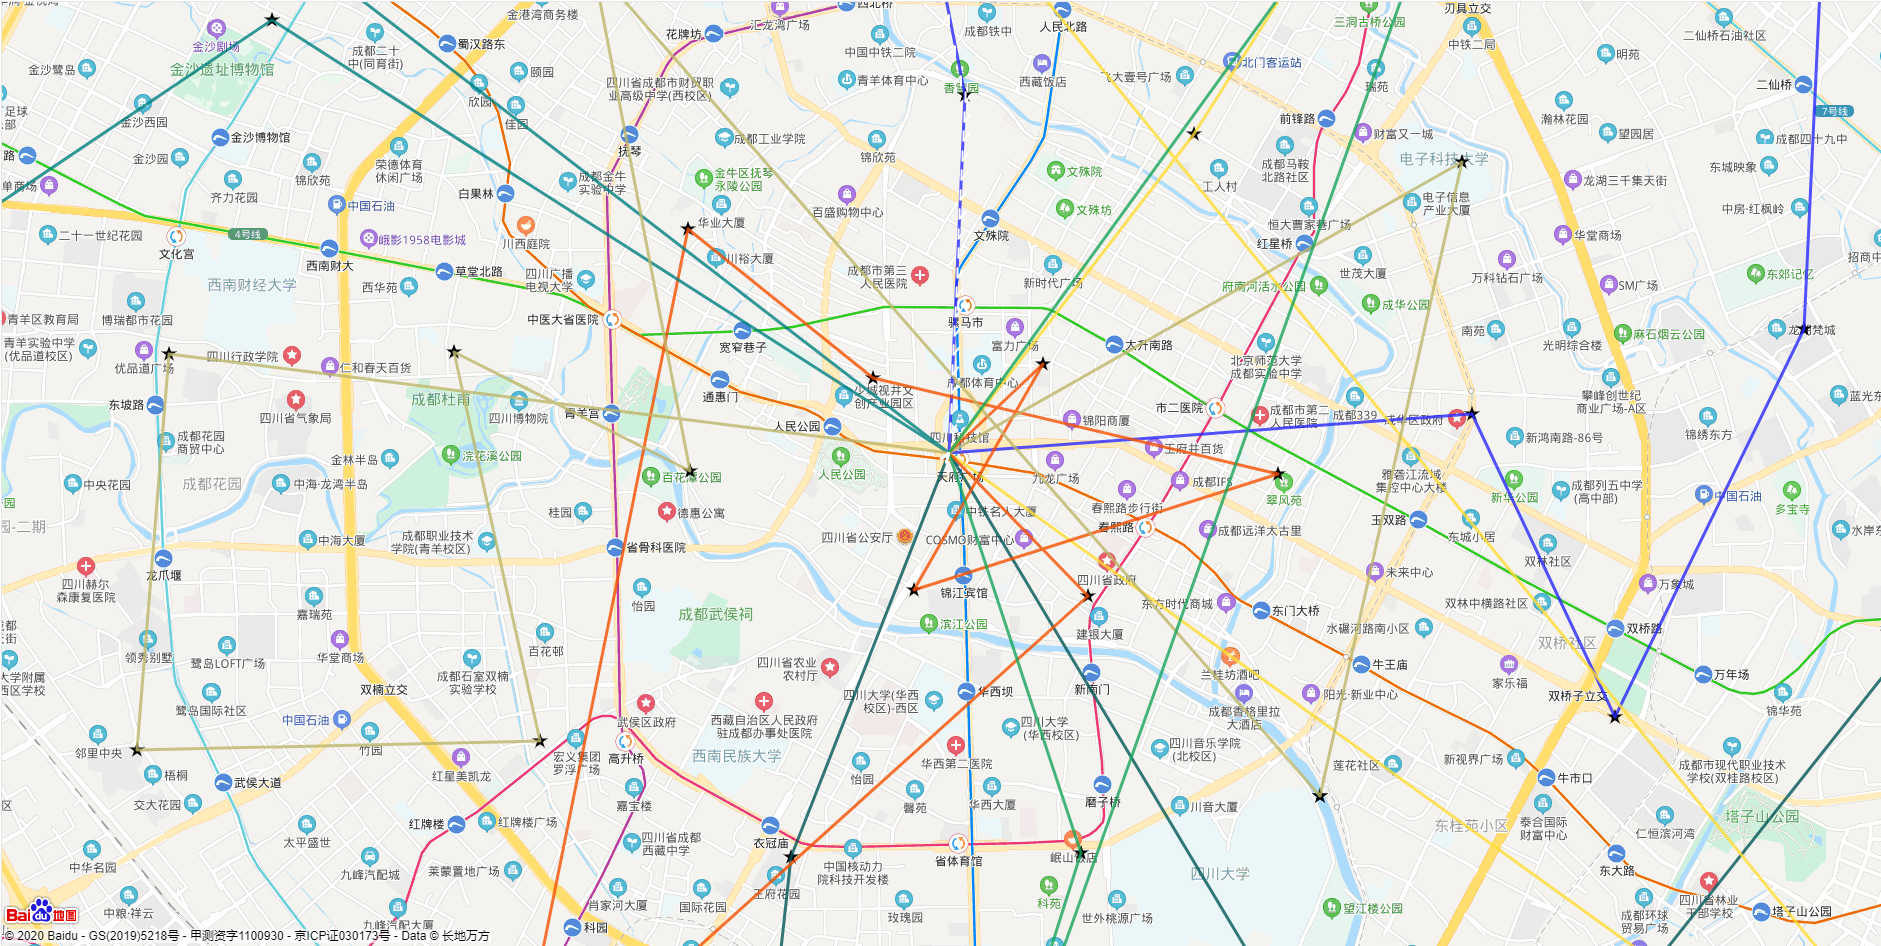
\includegraphics[width=6cm]{figures/cd_50_1.png}
				\caption{Routes Map 1}
			\end{minipage}%
		\end{subfigure}
		\begin{subfigure}[t]{0.45\textwidth}
			\begin{minipage}{6cm}
				\centering
				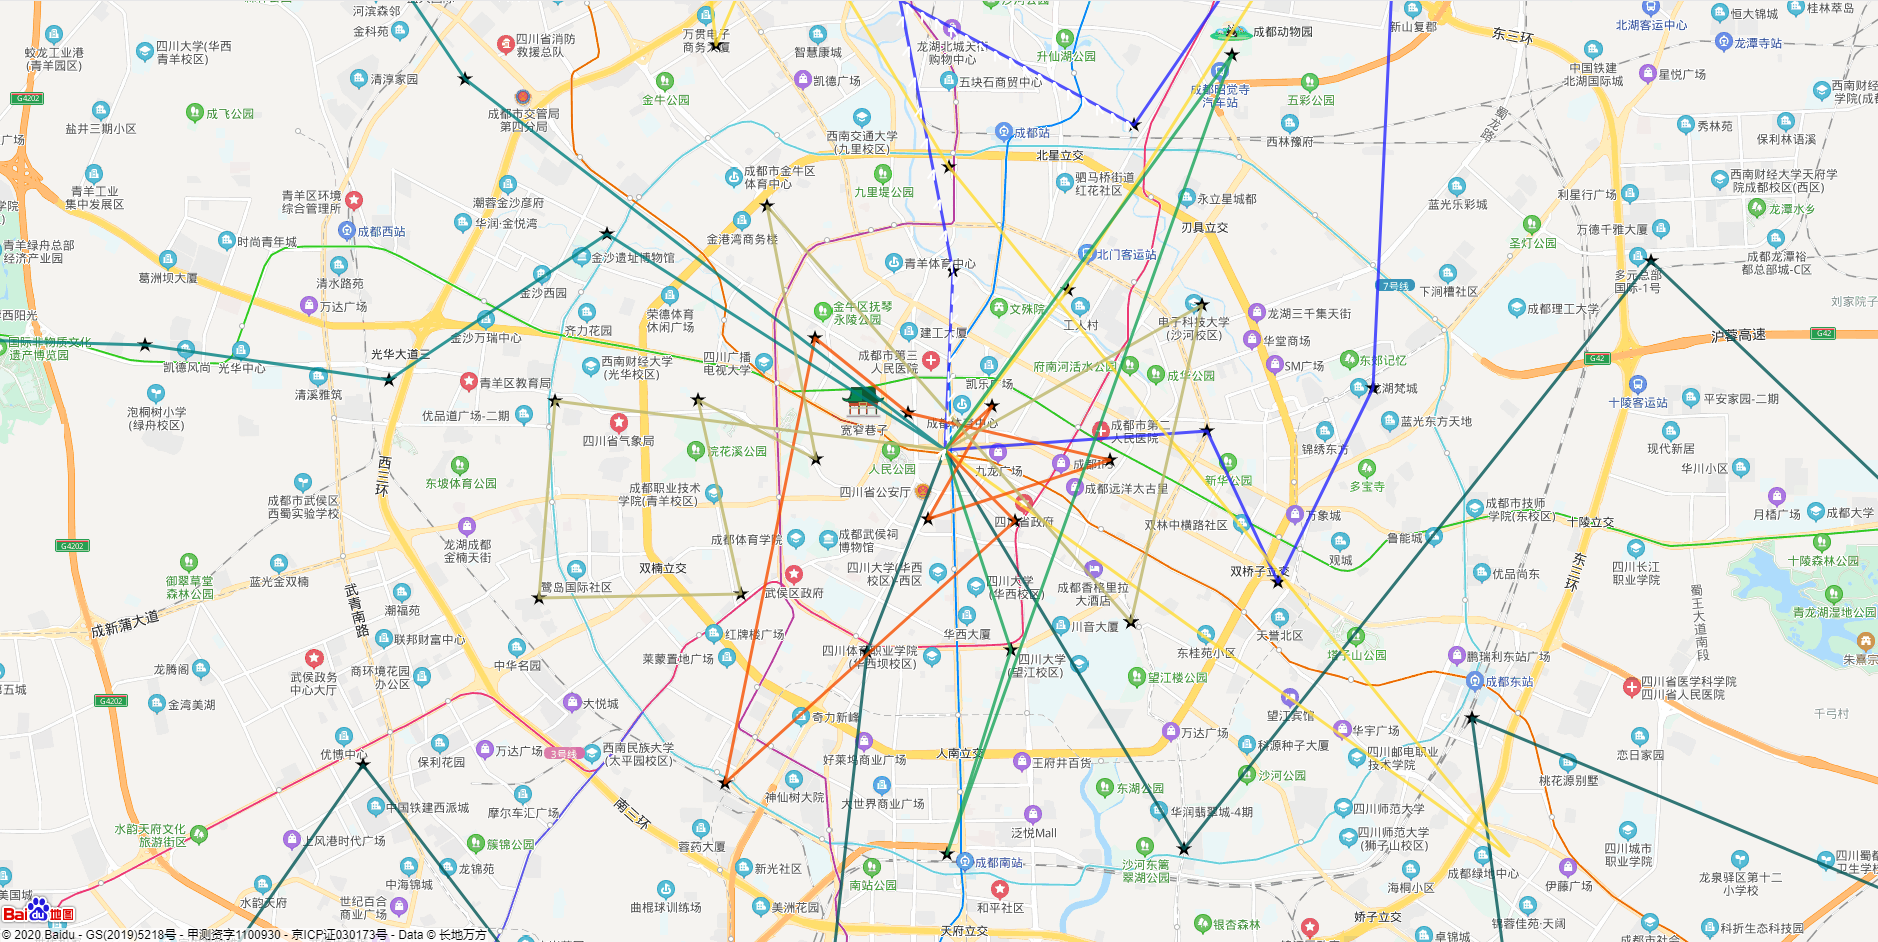
\includegraphics[width=6cm]{figures/cd_50_2.png}
				\caption{Routes Map 2}
			\end{minipage}
		\end{subfigure}
		\begin{subfigure}[t]{0.45\textwidth}
			\begin{minipage}{6cm}
				\centering
				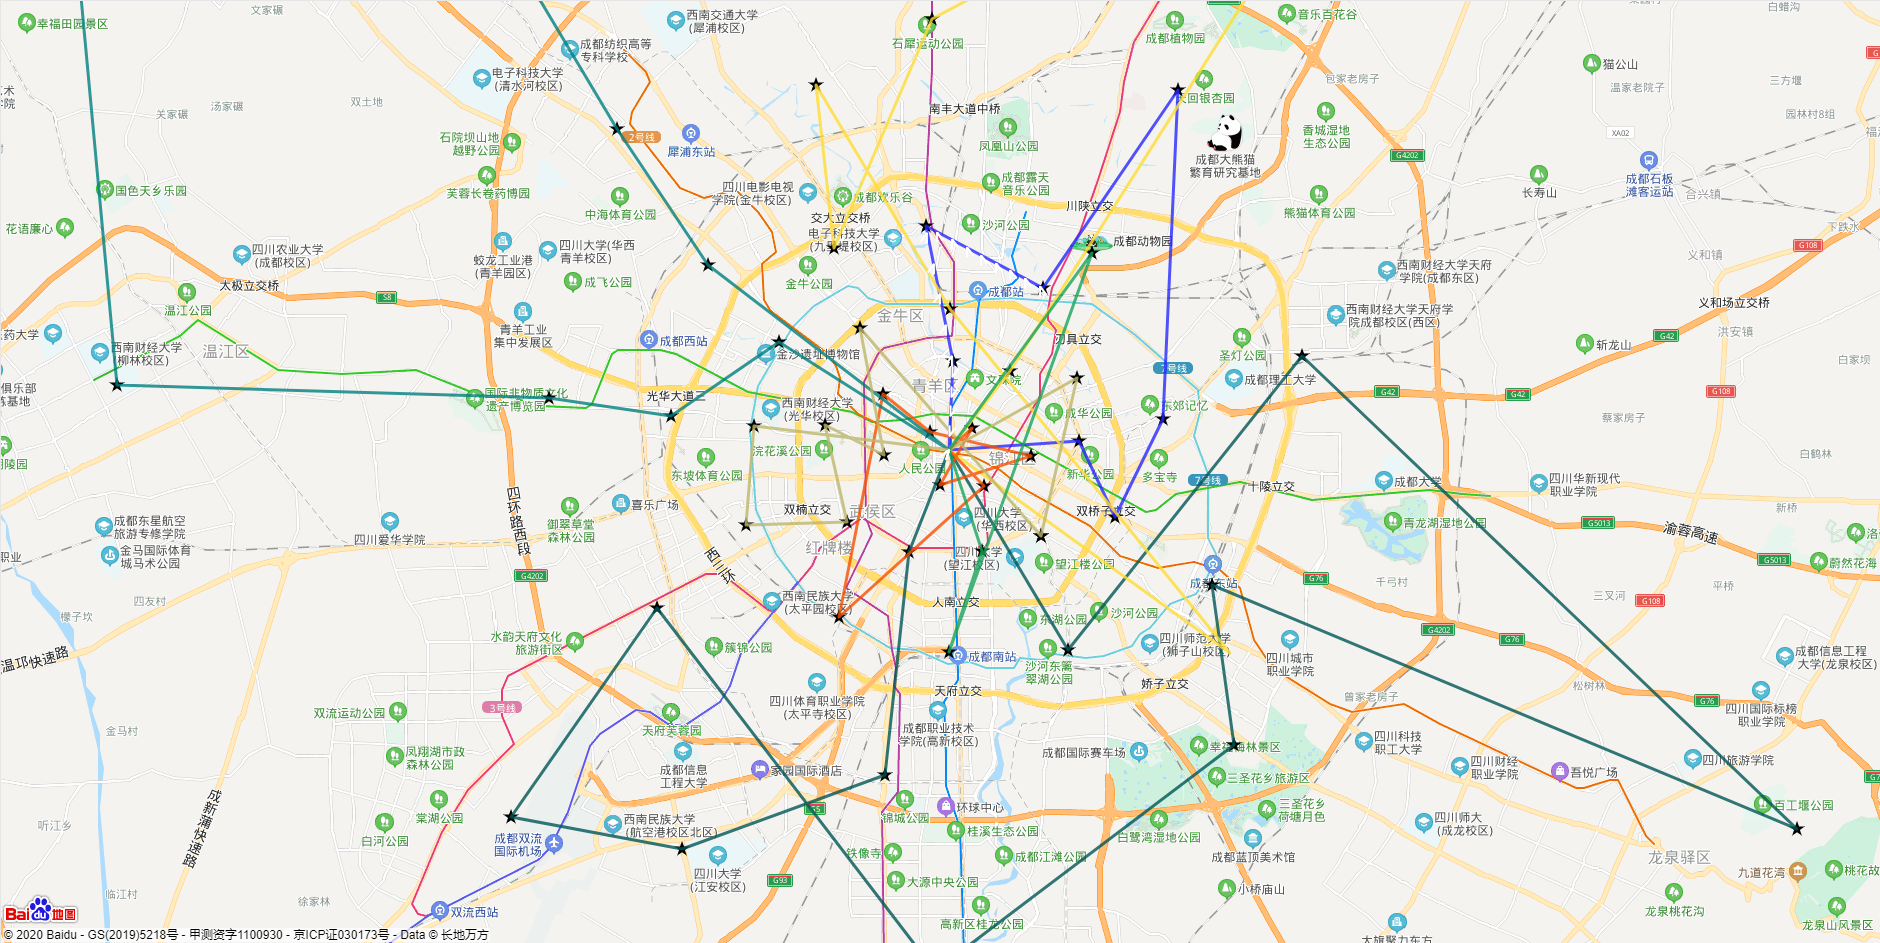
\includegraphics[width=6cm]{figures/cd_50_3.png}
				\caption{Routes Map 3}
			\end{minipage}%
		\end{subfigure}
		\begin{subfigure}[t]{0.45\textwidth}
			\begin{minipage}{6cm}
				\centering
				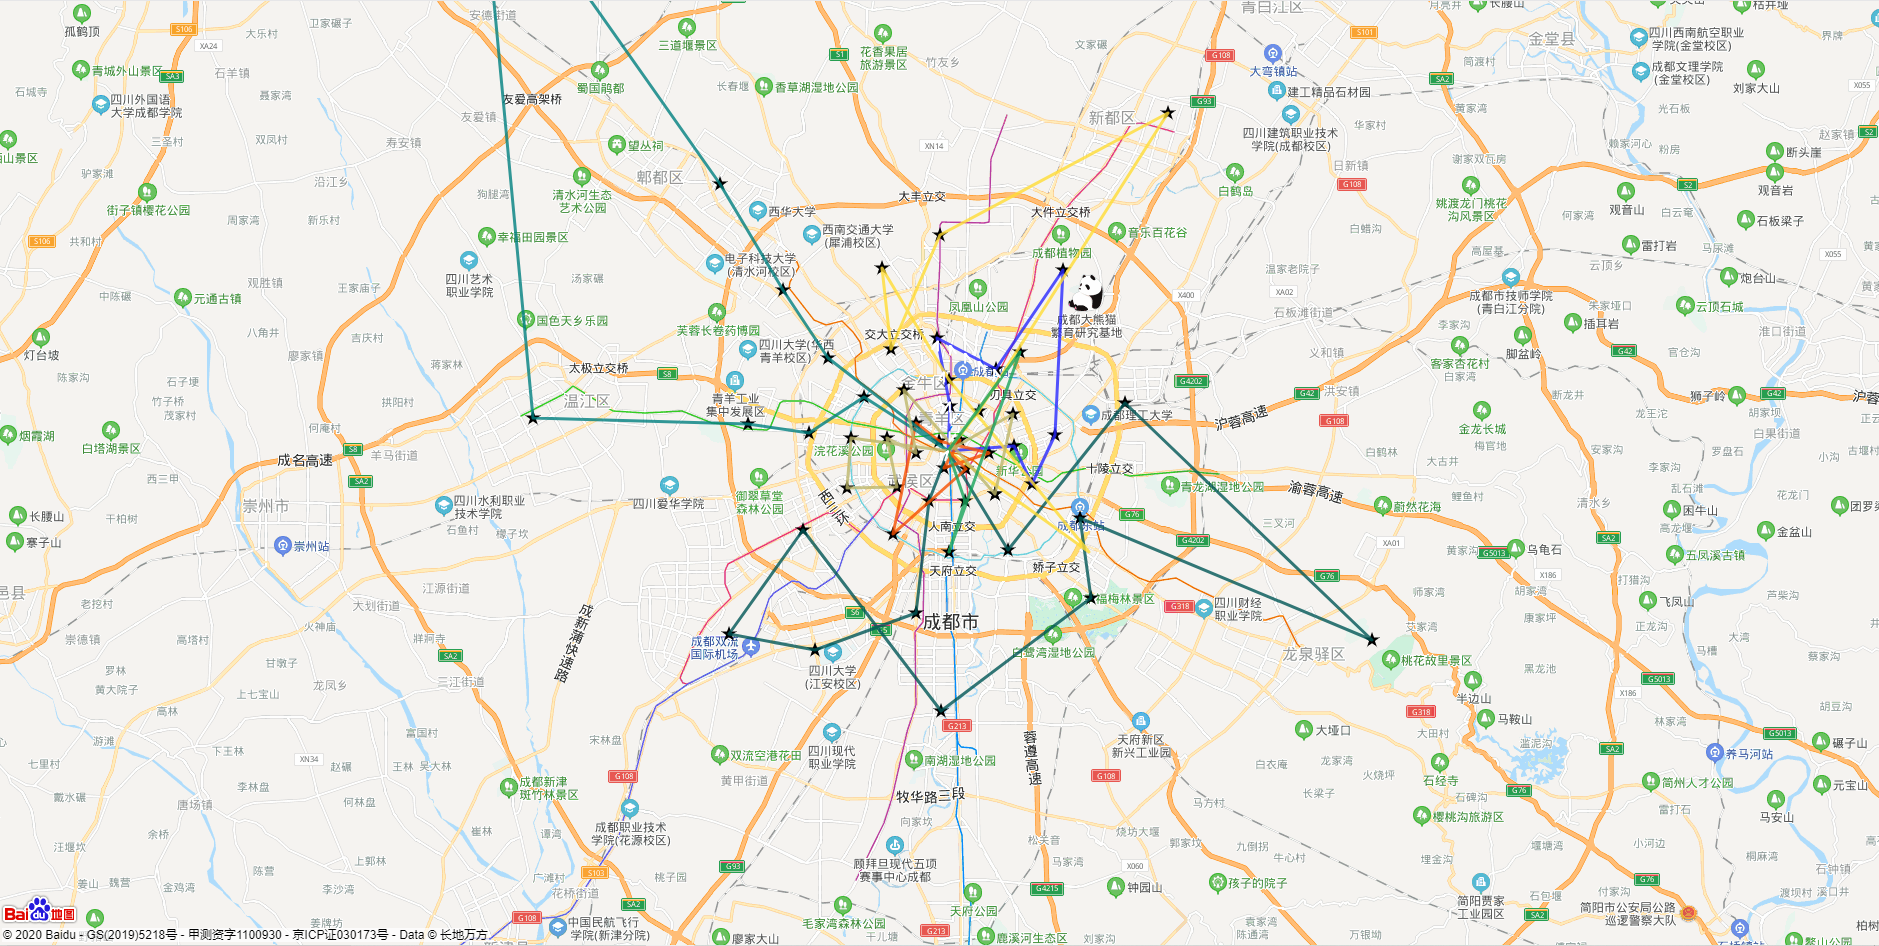
\includegraphics[width=6cm]{figures/cd_50_4.png}
				\caption{Routes Map 4}
			\end{minipage}
		\end{subfigure}
		\caption{$50$ Destinations Routes Maps with Different Scaling of Chengdu}
		\label{fig-cd-50}
		\end{figure}
	
	\item \textbf{Haikou-30}. When $k=30$, there are $3$ bus routes as Fig.\ref{fig-hk-30}.
	
		\begin{figure}[htbp]
		\centering
		\begin{subfigure}[t]{0.45\textwidth}
			\begin{minipage}{6cm}
				\centering
				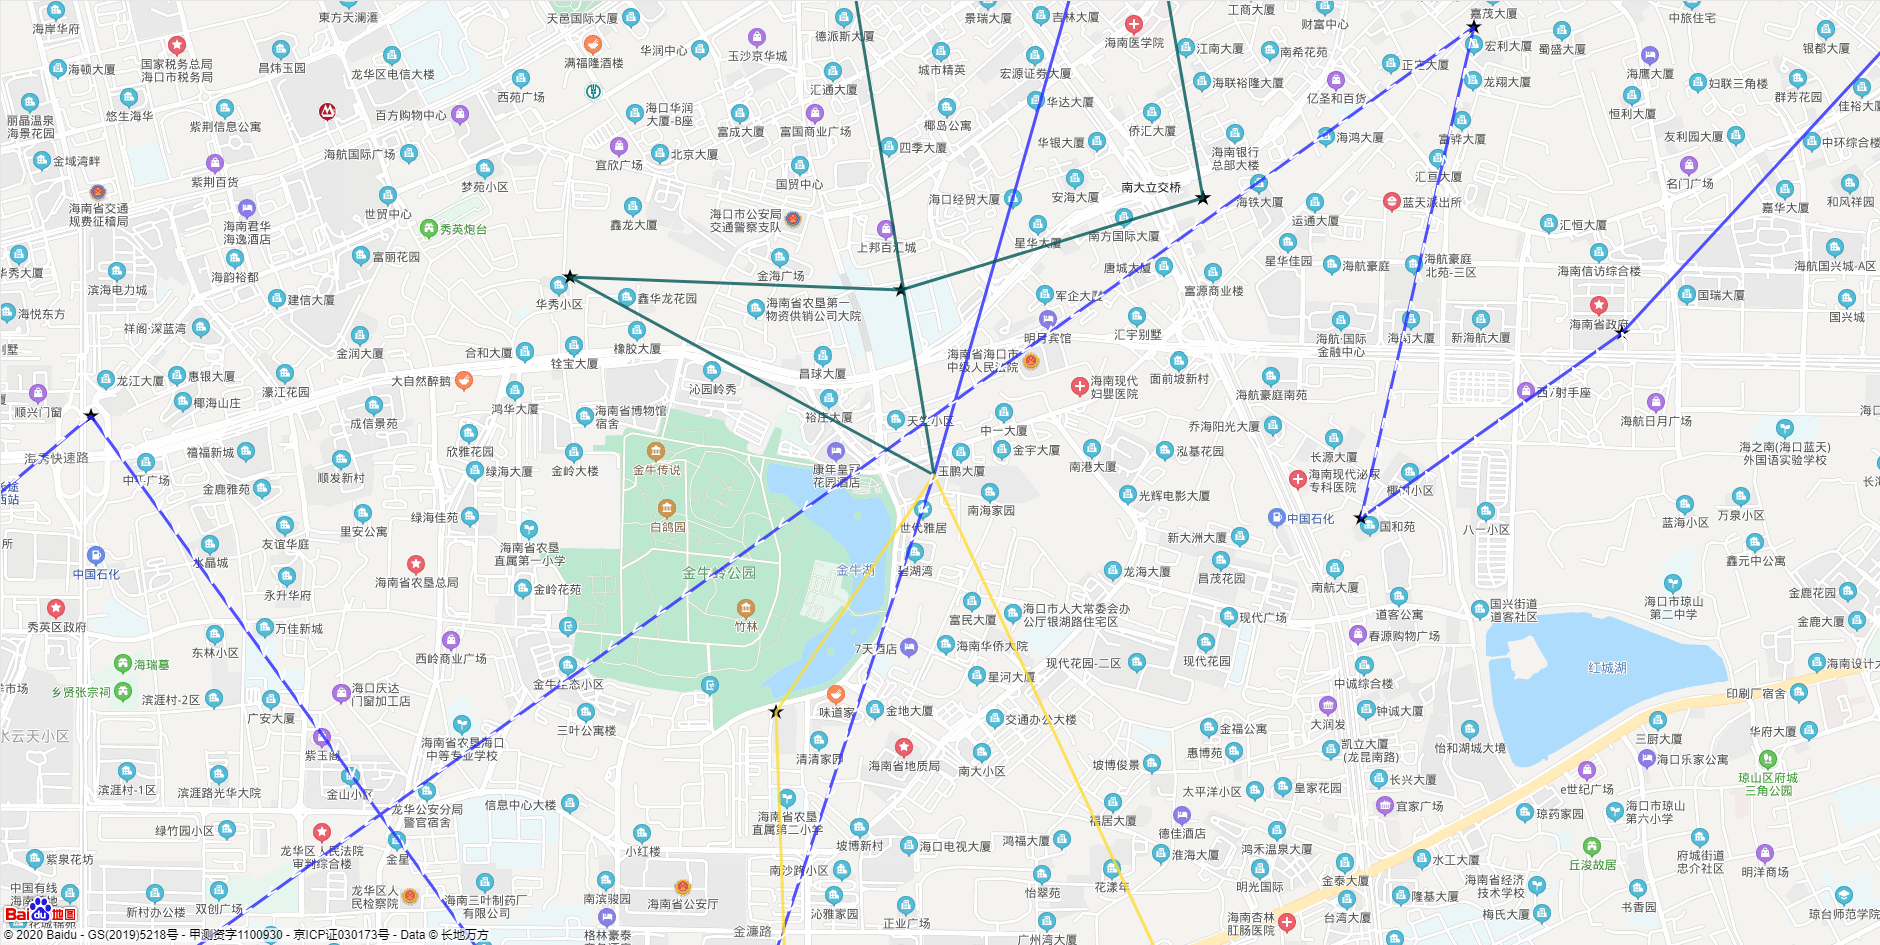
\includegraphics[width=6cm]{figures/hk_30_1.png}
				\caption{Routes Map 1}
			\end{minipage}%
		\end{subfigure}
		\begin{subfigure}[t]{0.45\textwidth}
			\begin{minipage}{6cm}
				\centering
				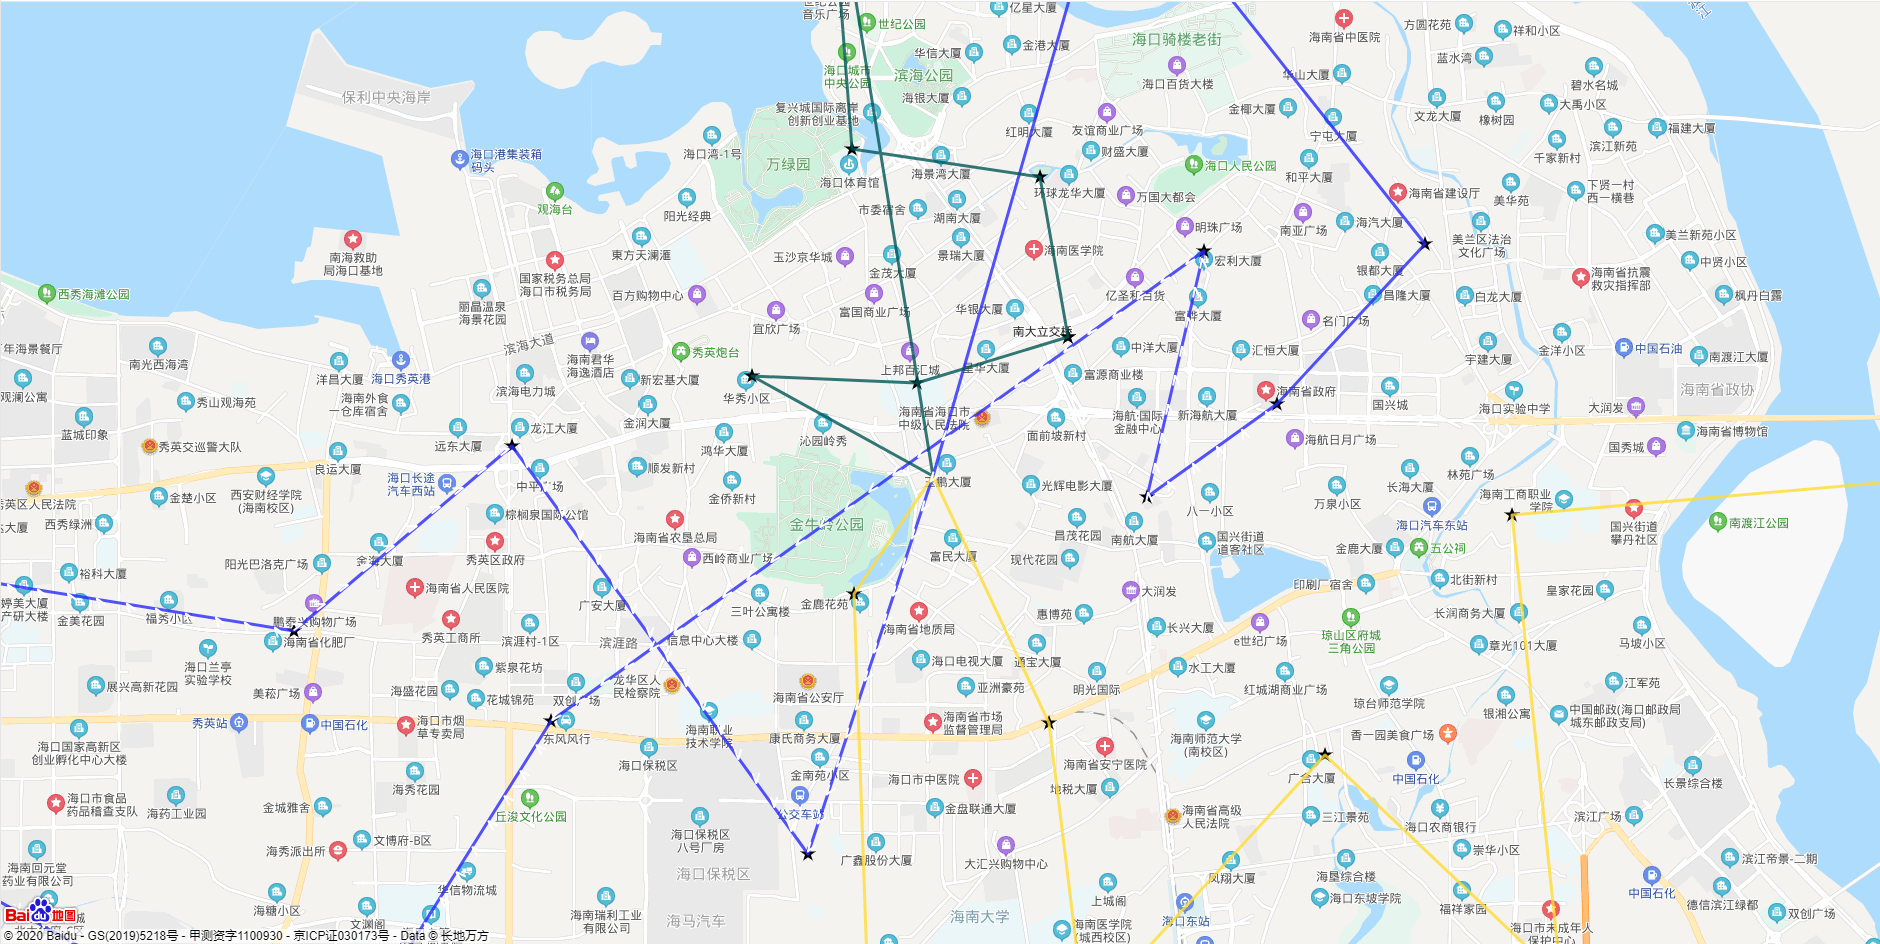
\includegraphics[width=6cm]{figures/hk_30_2.png}
				\caption{Routes Map 2}
			\end{minipage}
		\end{subfigure}
		\begin{subfigure}[t]{0.45\textwidth}
			\begin{minipage}{6cm}
				\centering
				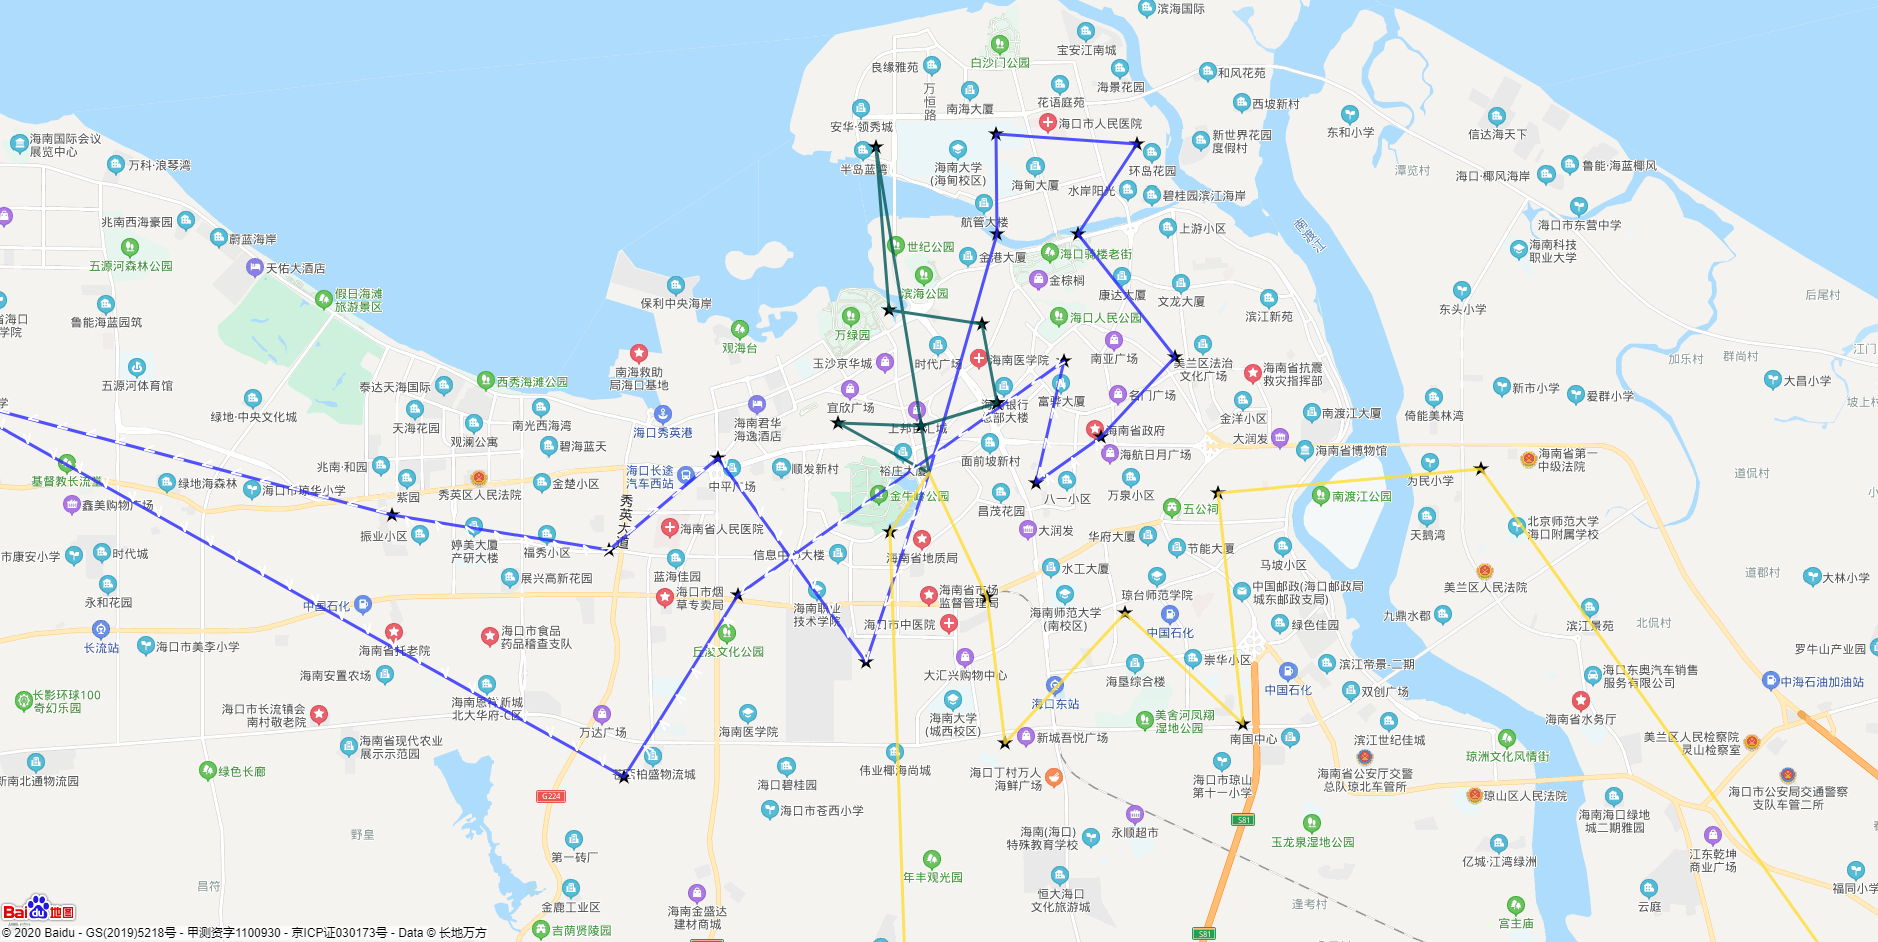
\includegraphics[width=6cm]{figures/hk_30_3.png}
				\caption{Routes Map 3}
			\end{minipage}%
		\end{subfigure}
		\begin{subfigure}[t]{0.45\textwidth}
			\begin{minipage}{6cm}
				\centering
				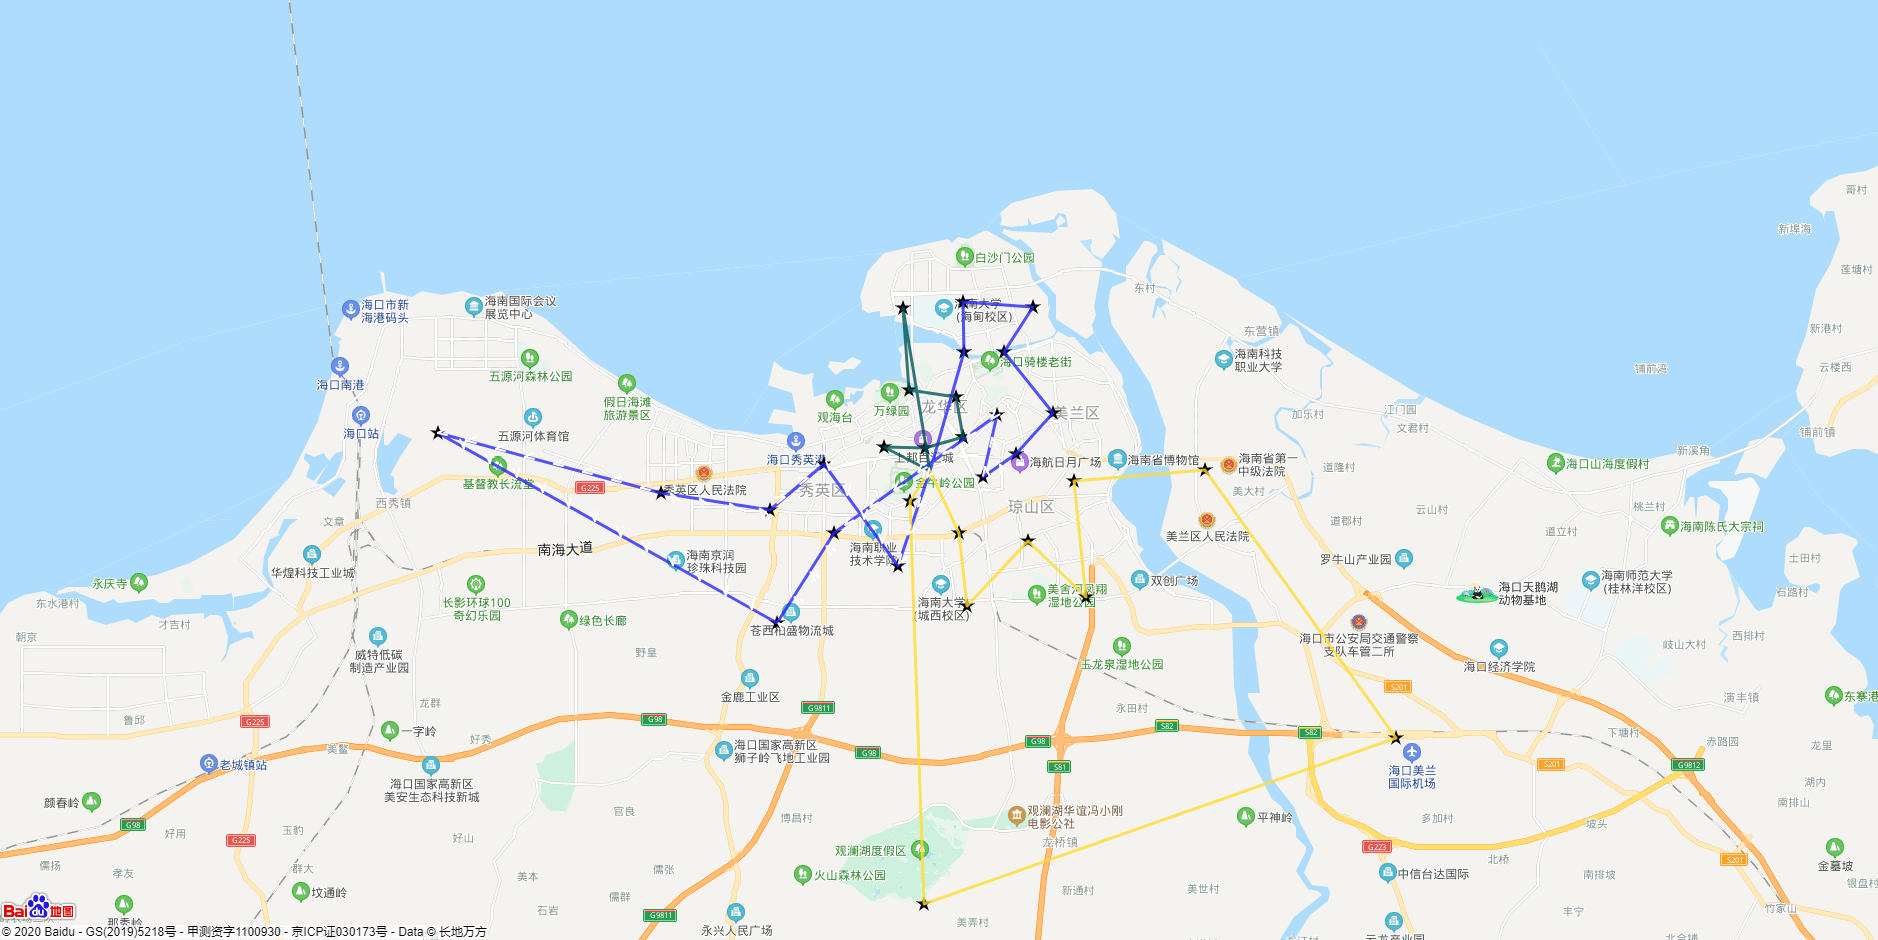
\includegraphics[width=6cm]{figures/hk_30_4.png}
				\caption{Routes Map 4}
			\end{minipage}
		\end{subfigure}
		\caption{$30$ Destinations Routes Maps with Different Scaling of Haikou}
		\label{fig-hk-30}
	\end{figure}
	
	\item \textbf{Haikou-50}. When $k=50$, there are $5$ bus routes as Fig.\ref{fig-hk-50}.
	
	\begin{figure}[htbp]
		\centering
		\begin{subfigure}[t]{0.45\textwidth}
			\begin{minipage}{6cm}
				\centering
				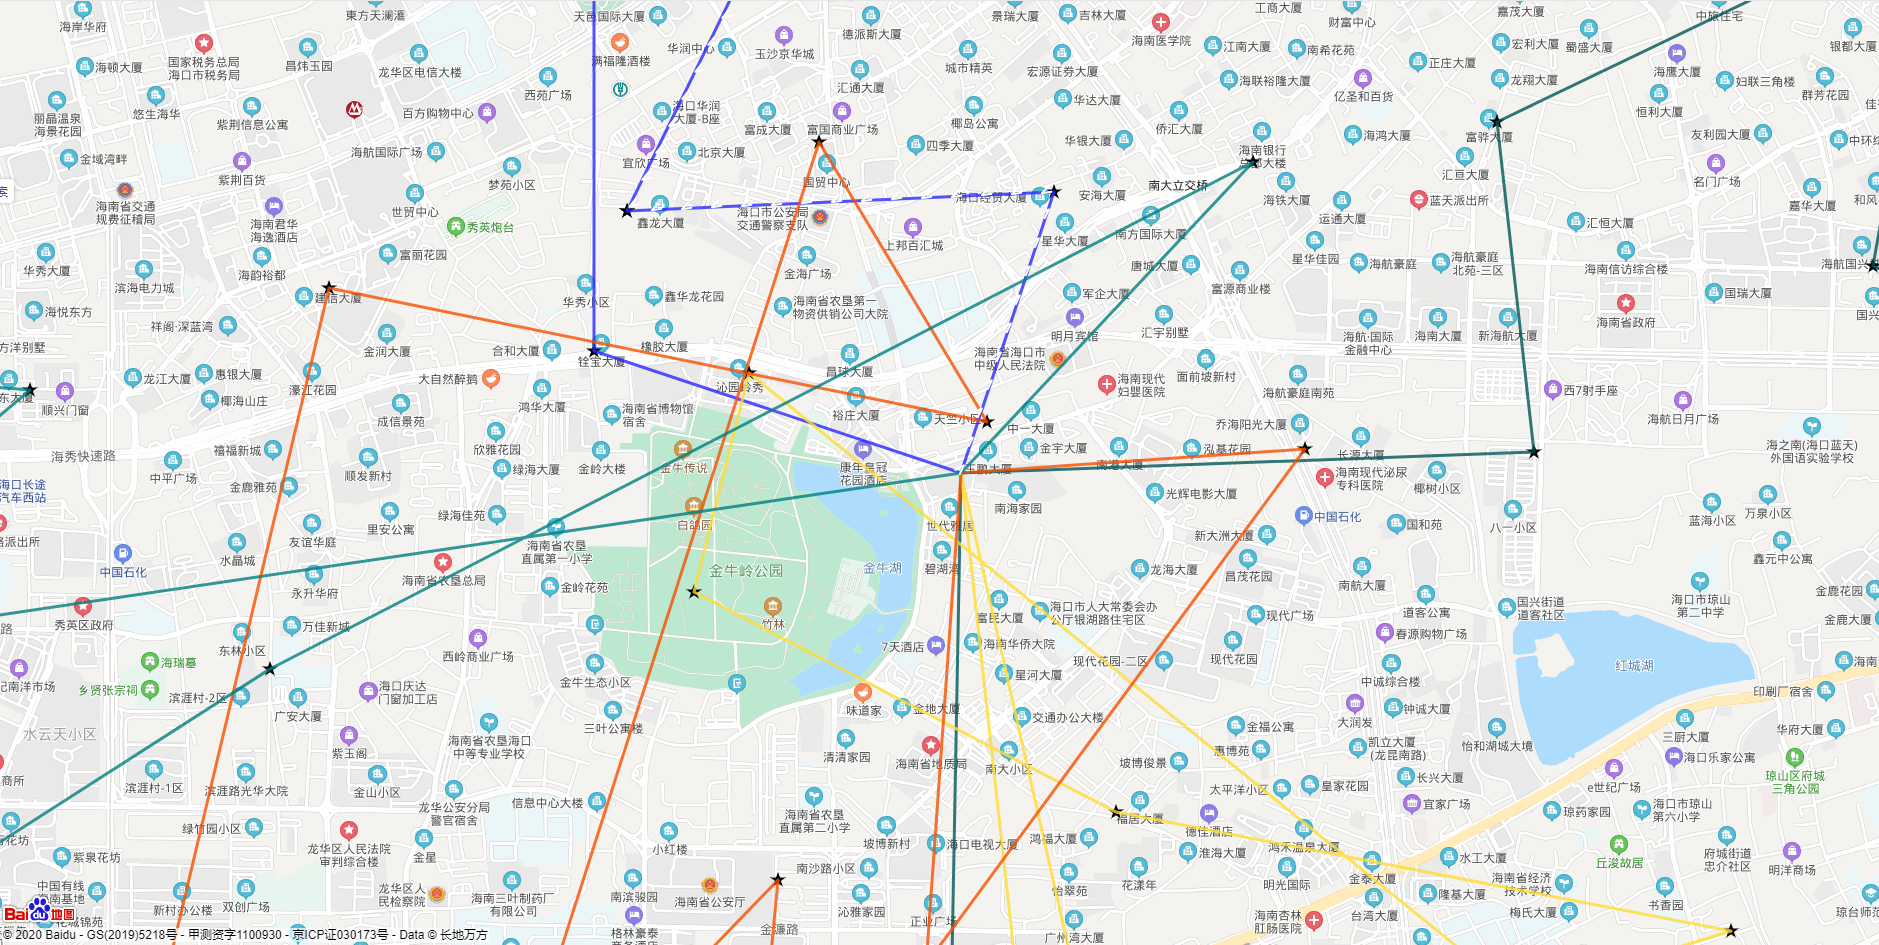
\includegraphics[width=6cm]{figures/hk_50_1.png}
				\caption{Routes Map 1}
			\end{minipage}%
		\end{subfigure}
		\begin{subfigure}[t]{0.45\textwidth}
			\begin{minipage}{6cm}
				\centering
				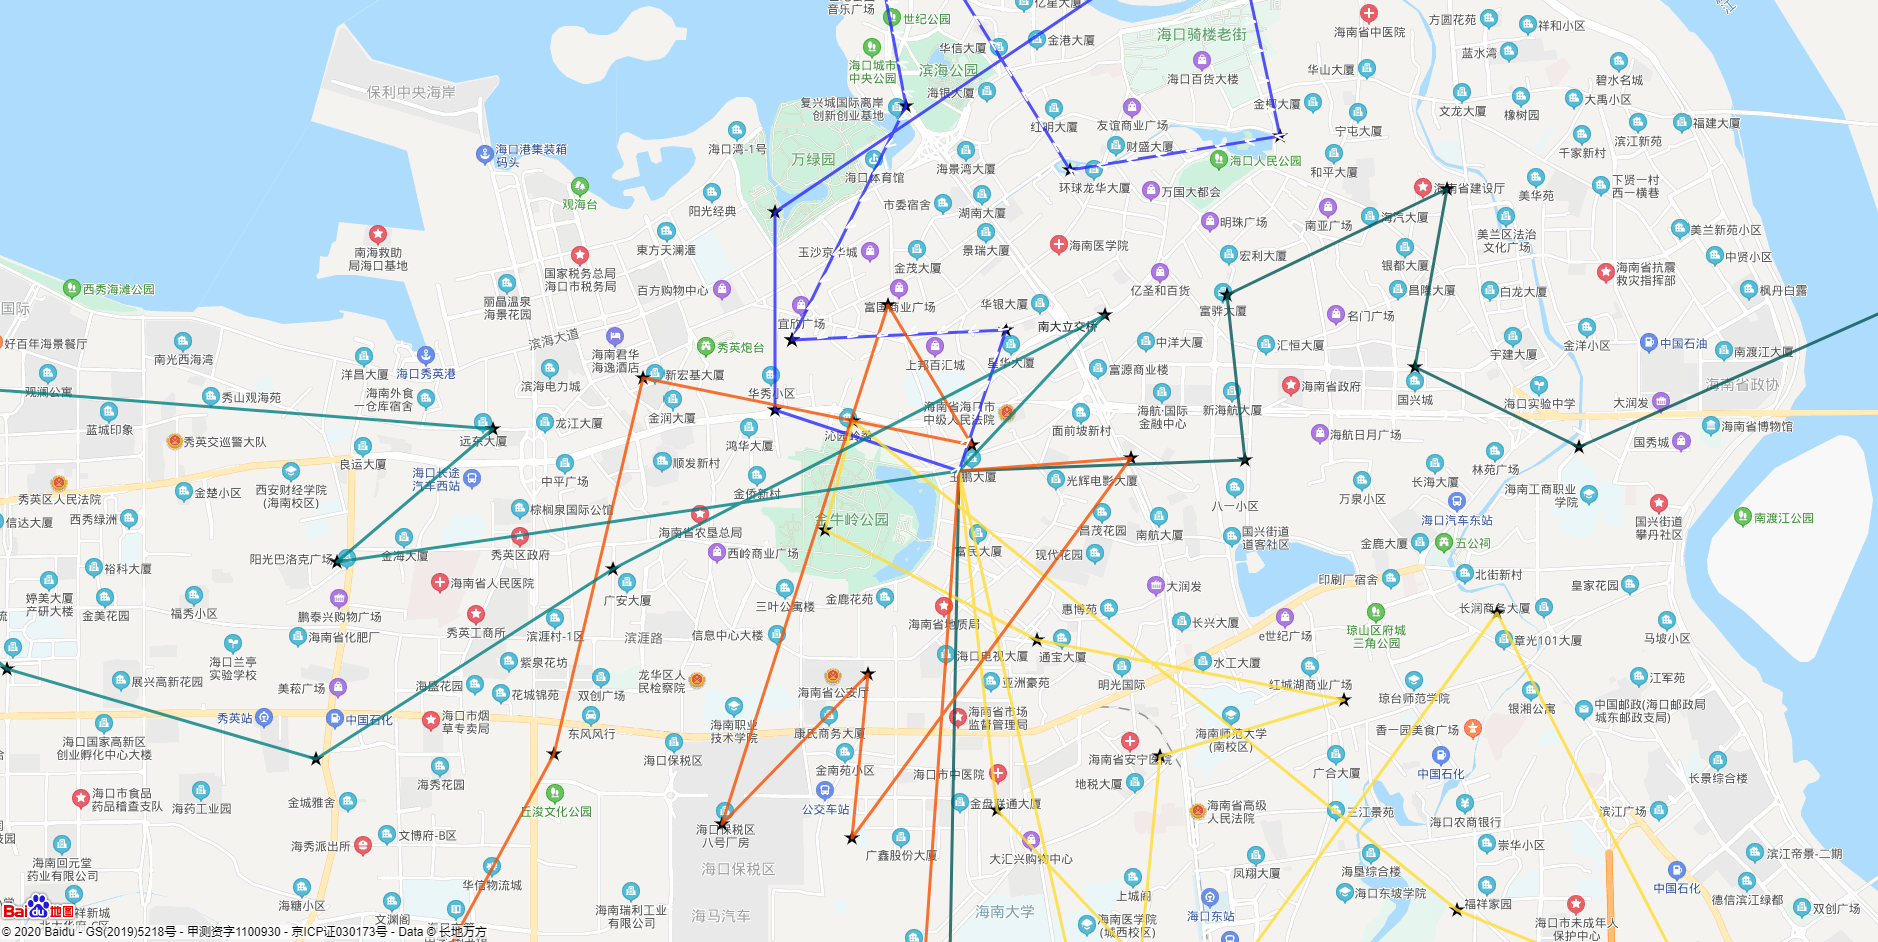
\includegraphics[width=6cm]{figures/hk_50_2.png}
				\caption{Routes Map 2}
			\end{minipage}
		\end{subfigure}
		\begin{subfigure}[t]{0.45\textwidth}
			\begin{minipage}{6cm}
				\centering
				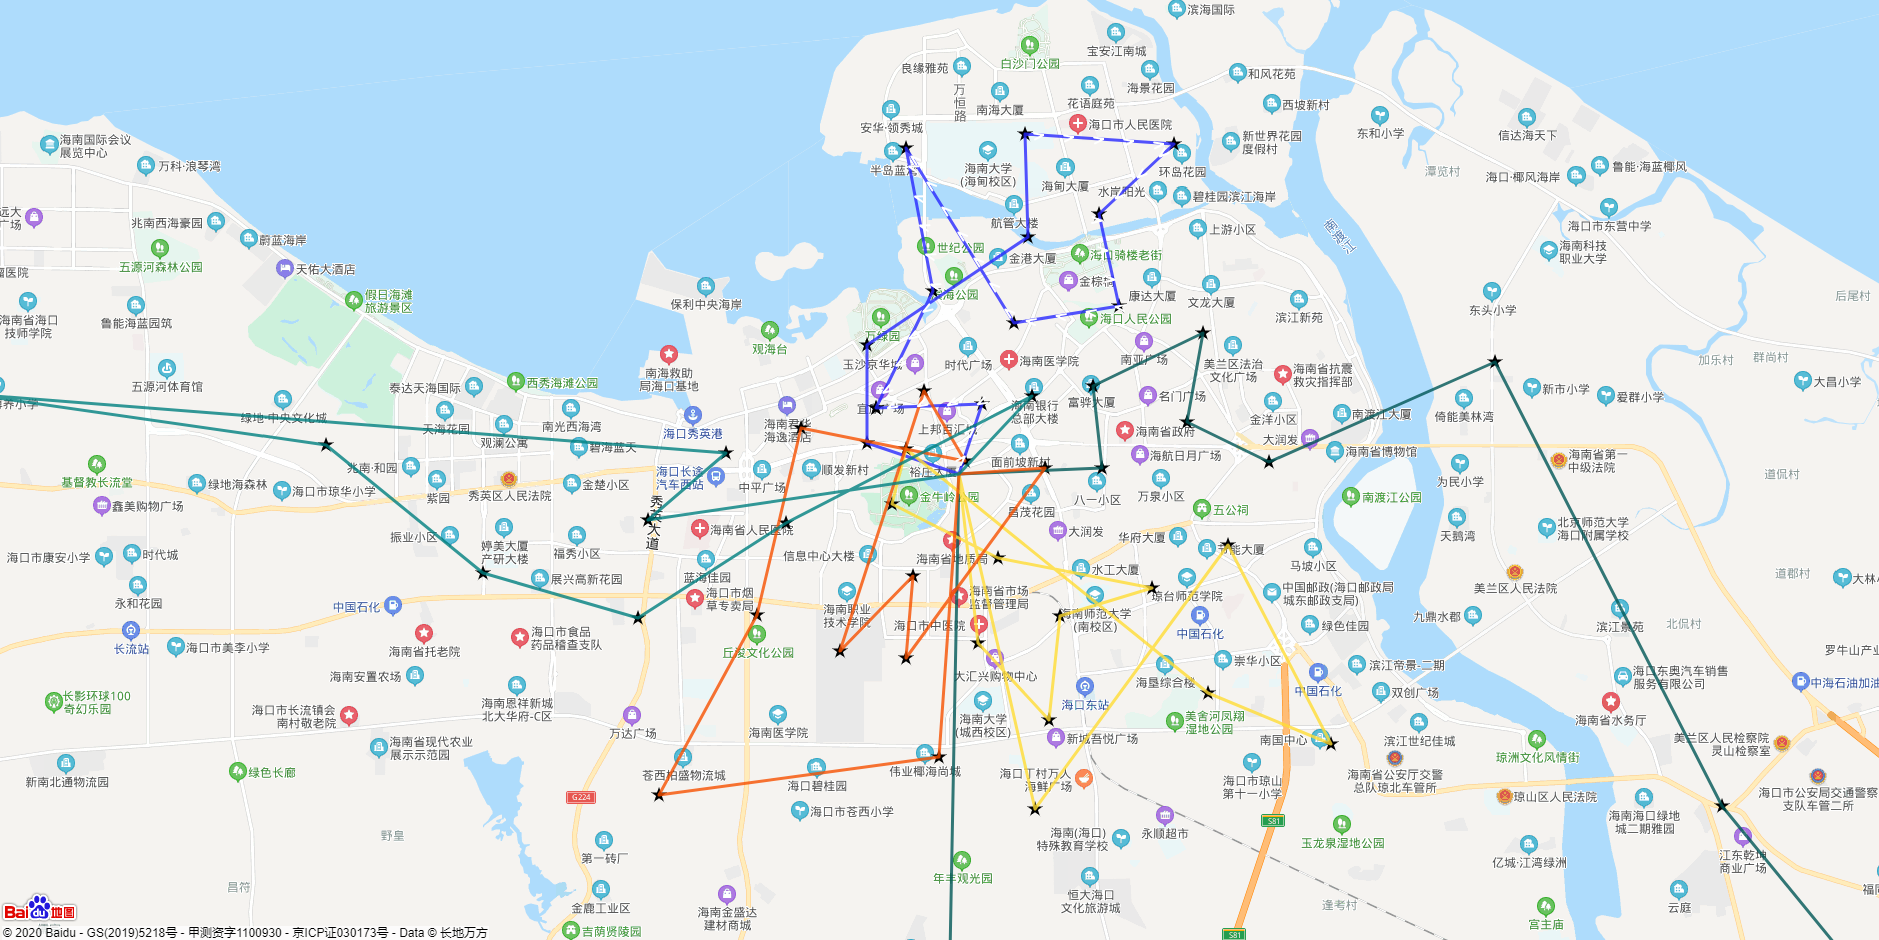
\includegraphics[width=6cm]{figures/hk_50_3.png}
				\caption{Routes Map 3}
			\end{minipage}%
		\end{subfigure}
		\begin{subfigure}[t]{0.45\textwidth}
			\begin{minipage}{6cm}
				\centering
				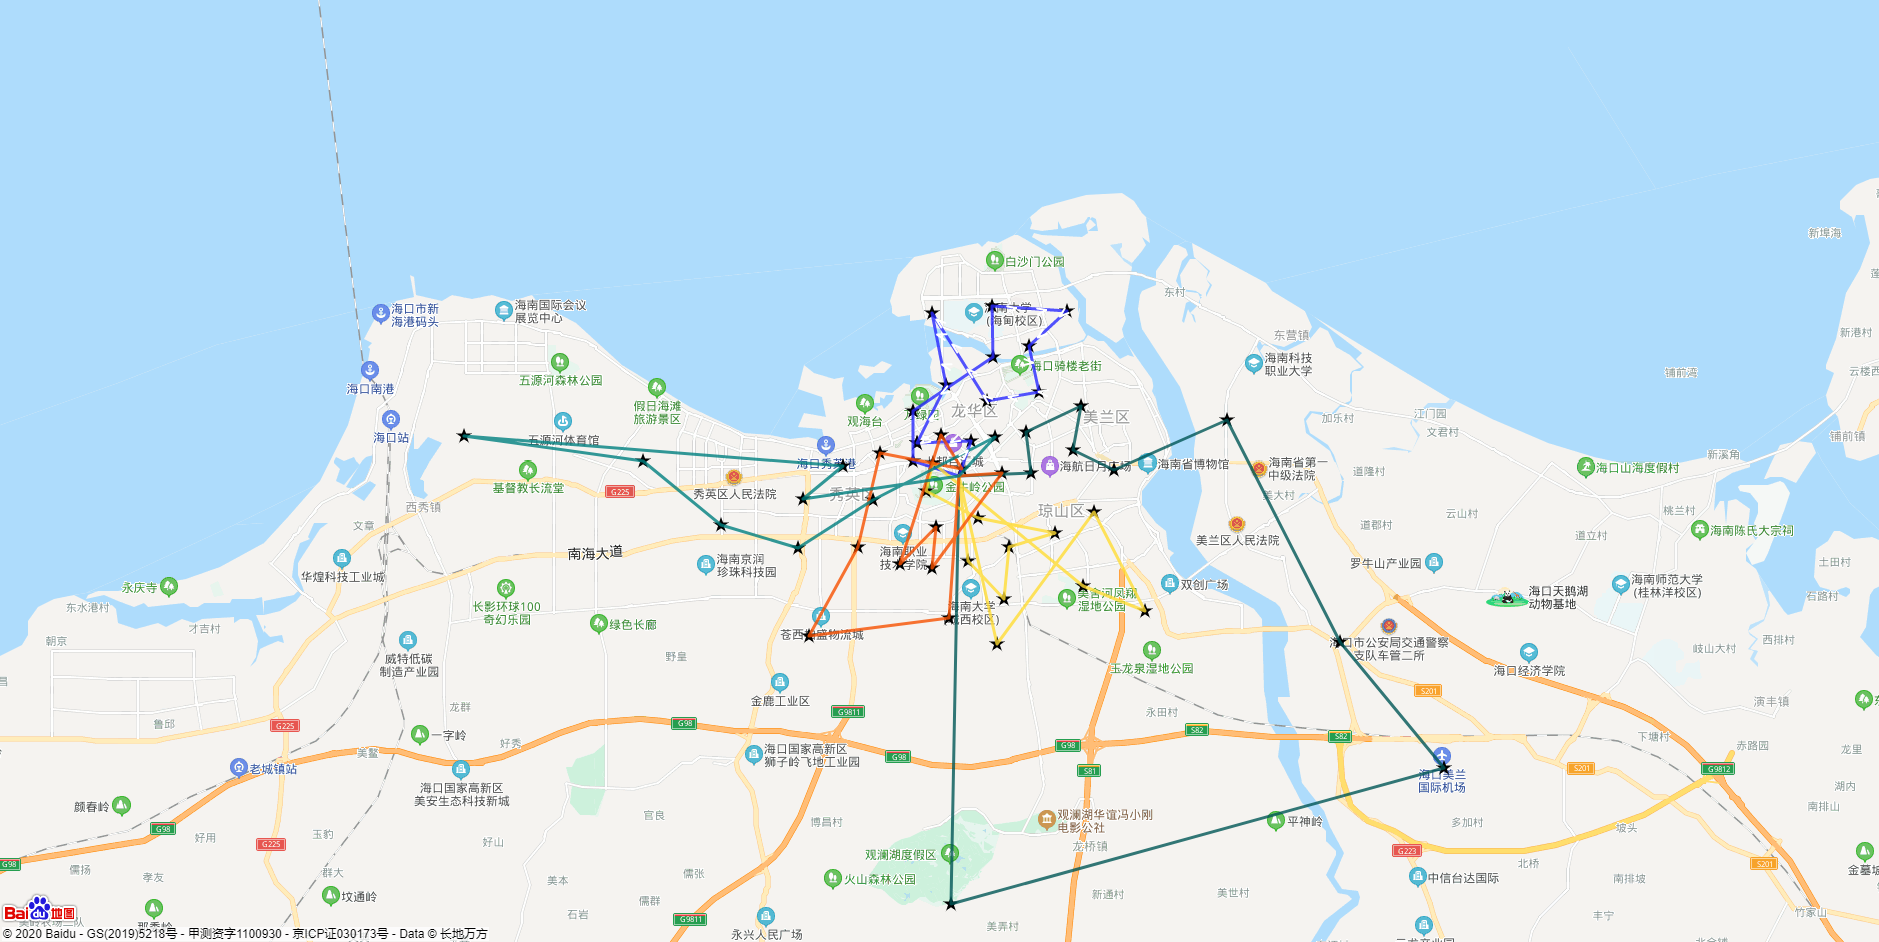
\includegraphics[width=6cm]{figures/hk_50_4.png}
				\caption{Routes Map 4}
			\end{minipage}
		\end{subfigure}
		\caption{$50$ Destinations Routes Maps with Different Scaling of Haikou}
		\label{fig-hk-50}
	\end{figure}
\end{itemize}

After route planning, we can get the final profit as follows:
	 	\begin{table}[htbp]
	\caption{Satisfaction $P(x)$ Change Table}
    	\begin{center}
		\begin{tabular}{|c|c|c|c|c|}
			\hline
			\diagbox[width=15em,trim=l]{City}{Bus Capacity} & $25$ & $30$ & $35$ & $45$ \\
			\hline
			Chengdu(30)			& $969927.94$ & $978391.28$ & $984389.47$ & $992320.52$ \\
			\hline
			Chengdu(50)			& $973702.95$ & $982240.96$ & $988093.55$ & $996233.34$ \\
			\hline
			Haikou(30)			& $714509.57$ & $720148.41$ & $724208.64$ & $729559.07$ \\
			\hline
			Haikou(50)			& $715535.04$ & $721165.73$ & $725214.58$ & $730651.19$ \\
			\hline
		\end{tabular}
	   \end{center}
    	\label{tab-profit}
		\end{table}
	
And the visible graph it is as Fig.\ref{fig-profit}.

\begin{figure}[h]
	
	\centering
	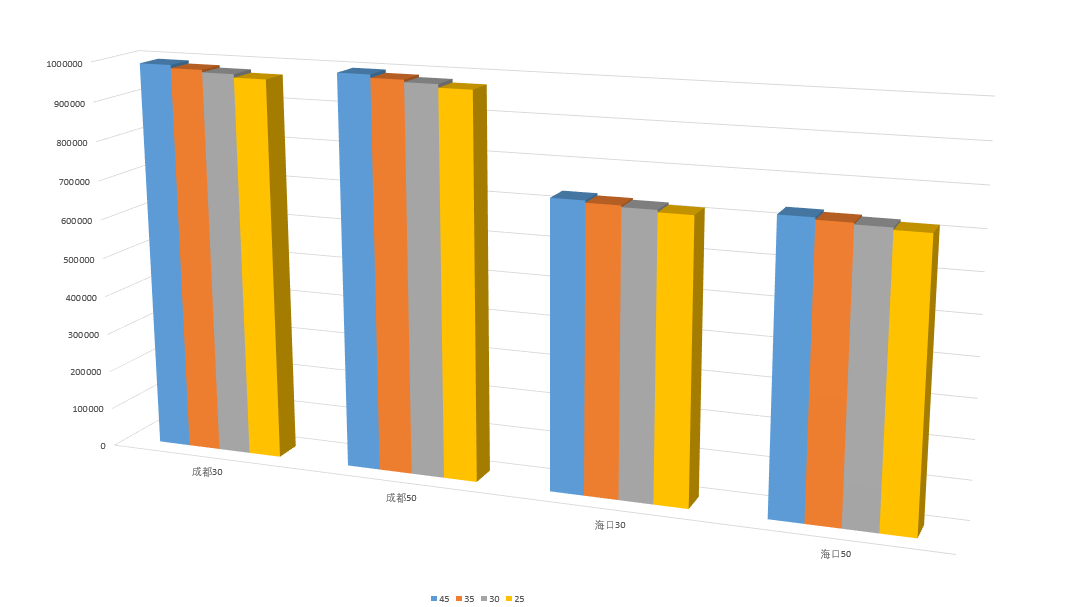
\includegraphics[width=12cm]{figures/profit.png}
	\caption{Visible Profit}
	\label{fig-profit}
	
\end{figure}

\subsection{Compare with Taxi}
We can compare our bus with taxi as Tab.\ref{tab-compare}.

	 	\begin{table}[htbp]
	\caption{Bus \& Taxi Comparing Table}
	\begin{center}
		\begin{tabular}{|c|c|c|}
			\hline
			\diagbox[width=15em,trim=l]{Cost Column}{Car Column} & Our Bus System & Taxi  \\
			\hline
			$c_f$(fuel cost per km)	    	& $2.211$ & $0.599$  \\
			\hline
			$c_r$			& $5.2$ & $6.5$  \\
			\hline
			Price($P(x)$)			& $8 + 0.9\times (x-2) +1.8$ & $8 + 3.3(x-2) + 6.6$  \\
			\hline
		\end{tabular}
	\end{center}
    	\label{tab-compare}
	\end{table}

It is obvious that on price column, our bus system has significant advantages. And although for each route, we have higher cost than taxi, our one bus has much more carry capacity than one taxi does. What's more, we  can attract much more orders. On the whole, our public transportation system creates more profits.

\vspace{10em}

\section*{Acknowledgements}
\begin{itemize}
	\item \textbf{Junxiang Cao}: In this project, we designed the model and algorithms to solve the bus booking problem and then analysed the performance of our algorithm. We made use of $k-means$ algorithms, graph($GA-TSP$) algorithms and other algorithms that we learned from the lecture. We met a lot of difficulties during these days, and we tried our best to get over them. For example, we used k-means algorithm to construct a destination stations graph to apply graph algorithms on it. After that, we designed a $GA-TSP$ algorithm to search for the feasible solution of the selections of bus routes. And also, in this project, we have learned a lot from each other in our team when communicating and arguing on problems. In the end, I would like to thank Professor Gao for teaching us so many useful algorithms and analyzing skills. We think we will benefit a lot from them in our future study.
	
	\vspace{1em}
	
	\item \textbf{Sen Li}: Before doing this project, I thought it was a programming-oriented code to implement the project. But after the beginning, I gradually realized that the difficulty lies more in the design and ideas of the algorithm, and many details that need to be finalized. We first discussed the implementation idea of this project together, and then divided the work. Throughout the process of completion, although we have separate divisions of labor, we have always maintained a positive attitude to discuss and solve problems, which has also allowed us to move forward steadily. This project has greatly exercised our ability to cooperate in completing tasks and is a very good exercise.
	
	\vspace{1em}
	
	\item \textbf{Shiqu Wu}: We've learned a lot about how to design and implement a middle project, and most important thing I've learned is teamwork.  My teammates are so great and so kind that they automatically  take the responsibility of  working out some difficult part of the project. They really let me understand the significance of trust in your teammates.  When I run into trouble,  rate of our project process is slowed.  But my teammates always encourage me to keep my own pace and don't worry about the other parts.  When using the \emph{CPLEX} to work out the optimal results,   I was stuck nearly for $3$ days for one simple mistakes.  And at first I don't know the computational ability of my computer and I push over half of the data into the CPLEX studio,  my computer soon crashed and I've try a lot of times to figure out the reasons.  It's really annoying that each time my computer crashed it take me a long time to reset all the other stuffs and open all the necessary materials.  It's the patience and the trust of my teammates that  push me through this difficulty.  In the end,  I want to thanks Pro. Gao for her kindness and patience about teaching us a lot of knowledge and a way to correctly treat the difficulty.  Thank you. 
\end{itemize}


%
% ---- Bibliography ----
%
% BibTeX users should specify bibliography style 'splncs04'.
% References will then be sorted and formatted in the correct style.
%
% \bibliographystyle{splncs04}
% \bibliography{mybibliography}
%
\begin{thebibliography}{8}
\bibitem{ref_article1}
Shijuan Hu. Research on multi traveling agent problem based on Improved Genetic Algorithm. Jiangnan University, 2019.

\bibitem{ref_url1}
\url{https://blog.csdn.net/weixin_43981664/article/details/104326573}.

\bibitem{ref_url2-taxi_fuel_cost}
\url{http://youjia.chemcp.com/sichuan/}

\bibitem{ref_url3-taxi_maintenance_cost}
\url{https://mbd.baidu.com/newspage/data/landingshare?context=%7B%22nid%22%3A%22news_9583968445811533527%22%2C%22ssid%22%3A%220761f69f%22%7D&pageType=1}
	
\bibitem{ref_url4-bus_fuel_price}
\url{http://www.xinhuanet.com/fortune/2019-03/01/c_1124178178.htm}

\bibitem{ref_url5-bus_fuel_cost}
\url{https://zhidao.baidu.com/question/553058868370993452.html}

\bibitem{ref_url6-bus_fixed_cost}
\url{https://www.carpenterbus.com/2015/01/annual-mini-bus-maintenance-costs/}




\end{thebibliography}
\end{document}
